\documentclass[11pt]{article}

% ============================================================
%  BBCN preprint scaffold (LaTeX)
%  Working scaffold: every number/figure/table is fixed and
%  reproducible from the companion repository (reproduce_all.py).
%  Final prose to be authored separately.
% ============================================================

\usepackage[utf8]{inputenc}
\usepackage[T1]{fontenc}
% \usepackage{lmodern} % optional; uncomment if installed
\usepackage[margin=1in]{geometry}
\usepackage{graphicx}
\usepackage{amsmath,amssymb}
\usepackage{booktabs}
\usepackage{authblk}
\usepackage{xcolor}
\usepackage{caption}
\usepackage{float}
\usepackage[hidelinks]{hyperref}
\captionsetup{font=small,labelfont=bf}

\definecolor{navy}{HTML}{1F3864}
\definecolor{authornote}{HTML}{9C6500}
\newcommand{\authornote}[1]{\par\noindent{\small\itshape\color{authornote}[Author note: #1]}\par}
% Internal to-dos: kept in source but suppressed in the posted/submitted build.
\renewcommand{\authornote}[1]{}

\title{\textbf{The Boolean Breast-Cancer Network (BBCN): structural controllability of cell-fate signalling and a bistable resistance--apoptosis switch}}
\author[1]{Aamer Iqbal Bhatti\thanks{Corresponding author. ORCID: 0000-0002-3373-3388.}}
\affil[1]{Department of Control and Instrumentation Engineering, King Fahd University of Petroleum and Minerals, Dhahran, Saudi Arabia}
\date{June 2026}

% All numerical values below come from results/numbers/numbers.tex, auto-generated
% by run_chunked.py over the full cohorts. The preprint never hard-codes a number.
% AUTO-GENERATED by run_chunked.py --emit — DO NOT EDIT BY HAND.
\newcommand{\BBCNACdeRankedIspyTwoStagepassApoptosisOn}{39}
\newcommand{\BBCNACdeRankedIspyTwoStagepassProliferationOff}{60}
\newcommand{\BBCNACdeRankedIspyTwoStagepassResistanceOff}{13}
\newcommand{\BBCNACdeRankedIspyTwoStagepassTerminal}{4}
\newcommand{\BBCNACdeRankedMetabricStagepassApoptosisOn}{33}
\newcommand{\BBCNACdeRankedMetabricStagepassProliferationOff}{61}
\newcommand{\BBCNACdeRankedMetabricStagepassResistanceOff}{7}
\newcommand{\BBCNACdeRankedMetabricStagepassTerminal}{1}
\newcommand{\BBCNACdeRankedTcgaStagepassApoptosisOn}{31}
\newcommand{\BBCNACdeRankedTcgaStagepassProliferationOff}{65}
\newcommand{\BBCNACdeRankedTcgaStagepassResistanceOff}{14}
\newcommand{\BBCNACdeRankedTcgaStagepassTerminal}{4}
\newcommand{\BBCNACdeStabilizeIspyTwoStagepassApoptosisOn}{35}
\newcommand{\BBCNACdeStabilizeIspyTwoStagepassProliferationOff}{43}
\newcommand{\BBCNACdeStabilizeIspyTwoStagepassResistanceOff}{8}
\newcommand{\BBCNACdeStabilizeIspyTwoStagepassTerminal}{3}
\newcommand{\BBCNACdeStabilizeMetabricStagepassApoptosisOn}{29}
\newcommand{\BBCNACdeStabilizeMetabricStagepassProliferationOff}{40}
\newcommand{\BBCNACdeStabilizeMetabricStagepassResistanceOff}{4}
\newcommand{\BBCNACdeStabilizeMetabricStagepassTerminal}{1}
\newcommand{\BBCNACdeStabilizeTcgaStagepassApoptosisOn}{27}
\newcommand{\BBCNACdeStabilizeTcgaStagepassProliferationOff}{39}
\newcommand{\BBCNACdeStabilizeTcgaStagepassResistanceOff}{8}
\newcommand{\BBCNACdeStabilizeTcgaStagepassTerminal}{3}
\newcommand{\BBCNAStaticRankedIspyTwoIsoApoptosisOn}{81}
\newcommand{\BBCNAStaticRankedIspyTwoIsoProliferationOff}{94}
\newcommand{\BBCNAStaticRankedIspyTwoIsoResistanceOff}{8}
\newcommand{\BBCNAStaticRankedIspyTwoN}{988}
\newcommand{\BBCNAStaticRankedIspyTwoSeqAllThree}{3}
\newcommand{\BBCNAStaticRankedIspyTwoSeqApoptosisOn}{9}
\newcommand{\BBCNAStaticRankedIspyTwoSeqProliferationOff}{4}
\newcommand{\BBCNAStaticRankedIspyTwoSeqResistanceOff}{8}
\newcommand{\BBCNAStaticRankedMetabricIsoApoptosisOn}{85}
\newcommand{\BBCNAStaticRankedMetabricIsoProliferationOff}{95}
\newcommand{\BBCNAStaticRankedMetabricIsoResistanceOff}{4}
\newcommand{\BBCNAStaticRankedMetabricN}{1980}
\newcommand{\BBCNAStaticRankedMetabricSeqAllThree}{2}
\newcommand{\BBCNAStaticRankedMetabricSeqApoptosisOn}{5}
\newcommand{\BBCNAStaticRankedMetabricSeqProliferationOff}{2}
\newcommand{\BBCNAStaticRankedMetabricSeqResistanceOff}{4}
\newcommand{\BBCNAStaticRankedTcgaIsoApoptosisOn}{86}
\newcommand{\BBCNAStaticRankedTcgaIsoProliferationOff}{94}
\newcommand{\BBCNAStaticRankedTcgaIsoResistanceOff}{8}
\newcommand{\BBCNAStaticRankedTcgaN}{1082}
\newcommand{\BBCNAStaticRankedTcgaSeqAllThree}{3}
\newcommand{\BBCNAStaticRankedTcgaSeqApoptosisOn}{9}
\newcommand{\BBCNAStaticRankedTcgaSeqProliferationOff}{3}
\newcommand{\BBCNAStaticRankedTcgaSeqResistanceOff}{8}
\newcommand{\BBCNAStaticStabilizeIspyTwoIsoApoptosisOn}{87}
\newcommand{\BBCNAStaticStabilizeIspyTwoIsoProliferationOff}{91}
\newcommand{\BBCNAStaticStabilizeIspyTwoIsoResistanceOff}{5}
\newcommand{\BBCNAStaticStabilizeIspyTwoN}{988}
\newcommand{\BBCNAStaticStabilizeIspyTwoSeqAllThree}{2}
\newcommand{\BBCNAStaticStabilizeIspyTwoSeqApoptosisOn}{12}
\newcommand{\BBCNAStaticStabilizeIspyTwoSeqProliferationOff}{2}
\newcommand{\BBCNAStaticStabilizeIspyTwoSeqResistanceOff}{5}
\newcommand{\BBCNAStaticStabilizeMetabricIsoApoptosisOn}{89}
\newcommand{\BBCNAStaticStabilizeMetabricIsoProliferationOff}{91}
\newcommand{\BBCNAStaticStabilizeMetabricIsoResistanceOff}{3}
\newcommand{\BBCNAStaticStabilizeMetabricN}{1980}
\newcommand{\BBCNAStaticStabilizeMetabricSeqAllThree}{1}
\newcommand{\BBCNAStaticStabilizeMetabricSeqApoptosisOn}{6}
\newcommand{\BBCNAStaticStabilizeMetabricSeqProliferationOff}{1}
\newcommand{\BBCNAStaticStabilizeMetabricSeqResistanceOff}{3}
\newcommand{\BBCNAStaticStabilizeTcgaIsoApoptosisOn}{91}
\newcommand{\BBCNAStaticStabilizeTcgaIsoProliferationOff}{85}
\newcommand{\BBCNAStaticStabilizeTcgaIsoResistanceOff}{5}
\newcommand{\BBCNAStaticStabilizeTcgaN}{1082}
\newcommand{\BBCNAStaticStabilizeTcgaSeqAllThree}{2}
\newcommand{\BBCNAStaticStabilizeTcgaSeqApoptosisOn}{11}
\newcommand{\BBCNAStaticStabilizeTcgaSeqProliferationOff}{2}
\newcommand{\BBCNAStaticStabilizeTcgaSeqResistanceOff}{5}
\newcommand{\BBCNBKernelRankedIspyTwoFlipPct}{46}
\newcommand{\BBCNBKernelRankedIspyTwoKerDesigned}{430}
\newcommand{\BBCNBKernelRankedIspyTwoKerSuccess}{198}
\newcommand{\BBCNBKernelRankedIspyTwoTopNode}{PIK3CA}
\newcommand{\BBCNBKernelRankedMetabricFlipPct}{42}
\newcommand{\BBCNBKernelRankedMetabricKerDesigned}{890}
\newcommand{\BBCNBKernelRankedMetabricKerSuccess}{373}
\newcommand{\BBCNBKernelRankedMetabricTopNode}{PIK3CA}
\newcommand{\BBCNBKernelRankedTcgaFlipPct}{47}
\newcommand{\BBCNBKernelRankedTcgaKerDesigned}{428}
\newcommand{\BBCNBKernelRankedTcgaKerSuccess}{202}
\newcommand{\BBCNBKernelRankedTcgaTopNode}{PIK3CA}
\newcommand{\BBCNBKernelStabilizeIspyTwoFlipPct}{46}
\newcommand{\BBCNBKernelStabilizeIspyTwoKerDesigned}{430}
\newcommand{\BBCNBKernelStabilizeIspyTwoKerSuccess}{198}
\newcommand{\BBCNBKernelStabilizeIspyTwoTopNode}{PIK3CA}
\newcommand{\BBCNBKernelStabilizeMetabricFlipPct}{42}
\newcommand{\BBCNBKernelStabilizeMetabricKerDesigned}{890}
\newcommand{\BBCNBKernelStabilizeMetabricKerSuccess}{373}
\newcommand{\BBCNBKernelStabilizeMetabricTopNode}{PIK3CA}
\newcommand{\BBCNBKernelStabilizeTcgaFlipPct}{47}
\newcommand{\BBCNBKernelStabilizeTcgaKerDesigned}{428}
\newcommand{\BBCNBKernelStabilizeTcgaKerSuccess}{202}
\newcommand{\BBCNBKernelStabilizeTcgaTopNode}{PIK3CA}
\newcommand{\BBCNBRoutingSwitchIspyTwoApopPct}{51}
\newcommand{\BBCNBRoutingSwitchIspyTwoMixedPct}{23}
\newcommand{\BBCNBRoutingSwitchIspyTwoN}{988}
\newcommand{\BBCNBRoutingSwitchIspyTwoResistApopZ}{0.08}
\newcommand{\BBCNBRoutingSwitchIspyTwoResistSurvZ}{0.32}
\newcommand{\BBCNBRoutingSwitchIspyTwoSurvPct}{25}
\newcommand{\BBCNBRoutingSwitchIspyTwoSurvUncoupledPct}{89}
\newcommand{\BBCNBRoutingSwitchIspyTwoUPct}{26}
\newcommand{\BBCNBRoutingSwitchMetabricApopPct}{48}
\newcommand{\BBCNBRoutingSwitchMetabricMixedPct}{22}
\newcommand{\BBCNBRoutingSwitchMetabricN}{1980}
\newcommand{\BBCNBRoutingSwitchMetabricResistApopZ}{0.11}
\newcommand{\BBCNBRoutingSwitchMetabricResistSurvZ}{0.2}
\newcommand{\BBCNBRoutingSwitchMetabricSurvPct}{29}
\newcommand{\BBCNBRoutingSwitchMetabricSurvUncoupledPct}{90}
\newcommand{\BBCNBRoutingSwitchMetabricUPct}{29}
\newcommand{\BBCNBRoutingSwitchTcgaApopPct}{50}
\newcommand{\BBCNBRoutingSwitchTcgaMixedPct}{14}
\newcommand{\BBCNBRoutingSwitchTcgaN}{1082}
\newcommand{\BBCNBRoutingSwitchTcgaResistApopZ}{0.32}
\newcommand{\BBCNBRoutingSwitchTcgaResistSurvZ}{0.8}
\newcommand{\BBCNBRoutingSwitchTcgaSurvPct}{36}
\newcommand{\BBCNBRoutingSwitchTcgaSurvUncoupledPct}{95}
\newcommand{\BBCNBRoutingSwitchTcgaUPct}{37}


\begin{document}
\maketitle

% ------------------------------------------------------------
\begin{abstract}
\noindent We model a breast tumour as a Boolean network of signalling pathways and pose therapy as a control problem: find minimal, druggable interventions that drive the network to a desired cell-fate phenotype as a genuine fixed point of the free dynamics, without permanently forcing any node. Two complementary analyses are reported (Figure~\ref{fig:arch}). In the first, a 135-node network is driven by a three-tier capped controller. Individual phenotypes are highly controllable (apoptosis 81--86\%, proliferation 94--95\% of patients across three cohorts), but achieving all three in sequence while preserving earlier gains is rare (2--3\%): the phenotypes share a dominant strongly-connected core (16 of 22 regulatory pathways), so they are individually feasible yet not jointly reachable. Feasibility does not imply reachability. In the second analysis, the apoptosis core is re-modelled as a bistable resistance--apoptosis switch built on AKT1--TP53 mutual antagonism, expressed as a delay-difference (Boolean-ARMA) system over $\mathrm{GF}(2)$ and run on a multi-timescale asynchronous schedule. Across three cohorts (TCGA-BRCA, METABRIC, I-SPY2; $N=1082/1980/988$) the switch routes about half of patients to the apoptotic attractor and a quarter to a survival attractor, and the survival-routed patients are 89--95\% in the uncoupled AKT--FOXO3a resistant state versus 26--37\% cohort-wide, a falsifiable prognostic alignment. The resistant attractor is held by hysteresis: survival-axis inhibition alone cannot flip it; only genotoxic input can. The nominated drug targets concentrate on the PI3K/AKT/mTOR axis and are robust across expression, signature, and phospho-protein front-ends. The model is a structural stratifier and drug-target nominator; it does not predict pathologic complete response, a limitation we trace to endpoint distance rather than signal quality.
\end{abstract}

% ------------------------------------------------------------
\section{Introduction}

Cancer arises from the distortion of the genetic information that regulates cellular pathways. This corruption dysregulates many signalling pathways at once and produces the cancer hallmarks: resistance, proliferation, and evasion of apoptosis. Because the pathways are coupled, a drug aimed at a single target is often less effective than expected; an effective therapy must act on several pathways together. This motivates a whole-network model in which each gene or protein is a Boolean node, ON or OFF, with an update rule drawn from the biological literature. We call this the Boolean Breast-Cancer Network (BBCN).

\subsection{Boolean models of cancer signalling and their control}
Boolean network modelling began with Kauffman's random Boolean networks~\cite{kauffman1969} and Thomas's logical description of regulatory systems as asynchronous automata~\cite{thomas1991}. Its predictive value for real biology was established by Albert and Othmer, whose Boolean model of the \emph{Drosophila} segment-polarity network reproduced wild-type and mutant expression patterns from logic alone~\cite{albert2003}. The appeal is practical: a Boolean model captures the qualitative logic of regulation without the kinetic rate constants that are rarely measurable, and every trajectory settles into an attractor that can be identified with a cell fate such as proliferation, quiescence, or apoptosis. Logic-based modelling of mammalian signalling was systematised by Saez-Rodriguez and colleagues~\cite{saez2009} and reviewed by Morris and co-workers~\cite{morris2010}, with community platforms such as the Cell Collective~\cite{helikar2012} and GINsim~\cite{naldi2018} making large logical models tractable to build and share.

In cancer, Boolean models have been used both to reproduce the hallmarks and to test interventions. Fumia and Martins built a network linking oncogenic pathways to carcinogenesis and targeted-therapy outcomes~\cite{fumia2013}. In breast cancer specifically, von der Heyde and colleagues reconstructed ERBB signalling and predicted cell-line-specific drug responses~\cite{vonderheyde2014}; Sgariglia and colleagues optimised therapeutic targets on a breast-cancer Boolean model~\cite{sgariglia2024}; and Taoma and colleagues modelled breast-cancer signalling to uncover mechanisms of drug synergy~\cite{taoma2024}. Gomez Tejeda Zanudo and colleagues used network models to elucidate drug-resistance mechanisms and to predict combination treatments in breast cancer~\cite{zanudo2017}.

The therapeutic question is then one of control: which nodes must be perturbed, and how, to steer the network from a pathological attractor to a desired one. The most influential structural answer is the stable-motif framework of Zanudo and Albert~\cite{zanudo2015}, which identifies from the network topology a minimal set of interventions that guarantee convergence to a target attractor; stable motifs are minimal strongly-connected components whose internal states form a partial fixed point, and the approach is packaged in widely-used tools~\cite{zanudo2013,rozum2022}. A related graph-theoretic route is feedback-vertex-set control, which selects determining nodes from the cycle structure of the network~\cite{fiedler2013}. A complementary algebraic tradition formulates Boolean control networks through the semi-tensor product of Cheng and colleagues~\cite{cheng2009}, which renders a Boolean network as a linear map over a lifted state space and supports formal controllability and global-stabilisation analyses, the latter developed recently by Rafimanzelat~\cite{rafimanzelat2025}. Probabilistic Boolean networks extend the formalism to stochastic regulation~\cite{shmulevich2002}. Finally, a patient-specific strand personalises a generic logical model to individual omics and simulates drug effects to nominate per-patient targets, developed by Montagud, Beal, Calzone and co-workers~\cite{montagud2022,beal2019}.

\subsection{Gap analysis}
The methods above are powerful, but two assumptions limit them on a network like BBCN, and together they define the gap this paper addresses.

The first gap is between feasibility and reachability. Most attractor-control methods, stable motifs and feedback-vertex-set control among them, establish \emph{feasibility}: they certify from the network structure that a target attractor exists and is, in principle, controllable. They do not test \emph{reachability} under a realistic budget, that is, whether a small, capped, non-accumulating set of druggable interventions actually drives a real patient's state to the target and holds it there as a genuine fixed point. Feasibility is a property of the network alone; reachability is a property of the network, the budget, and the patient together. The two can diverge, and on a strongly coupled network they do.

The second gap is the treatment of time. The standard Boolean update is synchronous or uniformly asynchronous, so every node advances on one clock. Yet the regulatory processes here span very different timescales: phosphorylation in seconds to minutes, protein turnover in hours, and transcription in hours to days. When a fast negative-feedback loop and a slow one are forced onto a single clock, the model can oscillate or settle into artefactual states with no biological counterpart. A control result built on such dynamics is not trustworthy for the apoptosis core, where fast survival signalling and slow transcriptional feedback are exactly what decide cell fate.

\subsection{Our approach}
This work addresses both gaps directly, in two linked setups on one network (Figure~\ref{fig:arch}). First, using a capped, no-forcing three-tier controller on three real cohorts, we test reachability rather than feasibility: we ask whether the cell-fate phenotypes can be reached and held together under a plausible drug budget. They cannot. The phenotypes are individually feasible and reachable but jointly near-mutually-exclusive, because they share a dominant strongly-connected core, so feasibility does not imply joint reachability. Second, we resolve the hardest phenotype, apoptosis, by re-modelling its core as a bistable switch expressed as a delay-difference system over $\mathrm{GF}(2)$, a Boolean analogue of an ARMA recurrence, in which the three process timescales enter as distinct update rates. To our knowledge this multi-timescale formulation is a novel way to embed biological timescale separation directly in the control of a patient-specific Boolean cancer model, and it is what lets the apoptosis core be steered where the whole-network controller could not.

This report makes four contributions. (i) A reproducible, capped, no-forcing three-tier controller for a 135-node breast-cancer Boolean network. (ii) A structural explanation of therapeutic failure: a dominant strongly-connected core makes the cell-fate phenotypes feasible individually but near-exclusive jointly. (iii) A bistable, multi-timescale (Boolean-ARMA) switch for the apoptosis core that routes patients coherently across three cohorts and explains targeted-therapy resistance as a hysteresis property. (iv) An honest validation: robust drug-target nomination on the PI3K/AKT/mTOR axis across three input front-ends, with an explicit null on pathologic-complete-response prediction traced to endpoint distance.

This work extends the author's earlier BBCN118 framework~\cite{bhatti2026}, a 118-node modular Boolean breast-cancer network whose central result was a Lyapunov-based pathway-decomposition theorem: under weak inter-pathway coupling, sequential pathway-wise stabilisation drives the network to a neighbourhood of the target. The present work tests that premise on the full network and three cohorts and finds that the weak-coupling regime does not cover the hard case, because the network is dominated by a strong cyclic core. The decomposition theorem is therefore the boundary this work pushes past; its proof is preserved in the earlier preprint and is restated for completeness in Appendix~\ref{app:theorem}. The bistable multi-timescale switch is new to the present work, while the forward-stabilisation kernel design is shared with BBCN118, here upgraded from the ranked reachability heuristic to an algebraic global-stabilisation test, with both methods retained and compared.

\subsection{Paper structure}
The rest of the paper is organised as follows. The Methods section describes the cohorts and binarisation, the two model setups, the three-tier controller and its kernel design, and the bistable multi-timescale switch. The Results section reports, in turn, the individual-versus-joint controllability gap (Section~\ref{sec:31}), the strongly-connected-core obstruction behind it (Section~\ref{sec:32}), the switch and its coherent patient routing (Section~\ref{sec:33}), the hysteresis nature of residual resistance and its drug interpretation (Section~\ref{sec:34}), the validation and the explicit limits of prediction (Section~\ref{sec:35}), and a head-to-head comparison of the two kernel methods and the static and dynamic controllers (Section~\ref{sec:comparison}). The Discussion places the findings against stable-motif and semi-tensor-product control theory. Three appendices make the work self-contained: Appendix~\ref{app:rules} lists the complete digital logic model, Appendix~\ref{app:flow} gives the flowcharts of the two kernel-design methods, and Appendix~\ref{app:theorem} restates the prior-work decomposition theorem whose boundary this paper maps. Every number, figure, and appendix regenerates from the companion repository with one command.

\begin{figure}[t]
\centering

\includegraphics[width=\textwidth]{figures/fig_arch.png}
\caption{\textbf{The two setups of BBCN.} A shared front end binarises patient mRNA. Setup~A (left) drives the full 135-node network with a three-tier capped controller (phenotype sequencing $\rightarrow$ cycle-level pathway selection $\rightarrow$ day-level forward-stabilisation kernel design) and yields the controllability obstruction. Setup~B (right) re-models the apoptosis core as a 9-node AKT1--TP53 bistable switch, expressed as a Boolean-ARMA / multirate system (fast/mid/slow boxes on a 1:5:25 asynchronous schedule) with an STP algebraic form, then applies the same forward-stabilisation kernel design per box. The apoptosis bottleneck found in Setup~A motivates Setup~B.}
\label{fig:arch}
\end{figure}

% ------------------------------------------------------------
\section{Methods}

\subsection{Cohorts and patient-state initialisation}
Patient states are derived from primary-tumour mRNA expression in three large public cohorts: TCGA-BRCA (1082 patients, RNA-seq), METABRIC (1980 patients, microarray), and I-SPY2 (988 patients, microarray; GEO GSE194040). The three cohorts were chosen to span different measurement platforms and different patient populations, so that any finding which holds across all three is unlikely to be an artefact of one assay or one centre. TCGA-BRCA and METABRIC are large primary-tumour reference cohorts on unrelated technologies, and I-SPY2 is a neoadjuvant trial cohort that also carries treatment annotation.

Each gene is converted to a Boolean value separately within each cohort. The activity score of a gene is its robust $z$-score, $(x-\mathrm{median})/(1.4826\cdot\mathrm{MAD})$, computed over all patients in that cohort, and the node is set ON when the score exceeds zero. The robust estimator is the default throughout. It uses the median and the median absolute deviation rather than the mean and the standard deviation, so a handful of extreme expression values, which are common in skewed RNA-sequencing data, cannot drag the threshold. Classic $z$-score and hard-median binarisation are retained only as alternatives for the sensitivity analysis, and the qualitative results do not depend on the choice.

Some nodes correspond to a signalling activity rather than to a single gene. For these, a curated multi-gene panel is reduced to one Boolean value by a majority vote: the node is ON when at least half of its panel genes are ON. The resulting Boolean vector, restricted to the network nodes, is the patient's initial state. The same front end feeds both setups, so Setup~A and Setup~B always see the identical binarised patient.

\subsection{The BBCN model and the two setups}
Two model instances are used and are kept clearly separated (Figure~\ref{fig:arch}). Setup~A is the 135-node network across 24 signalling pathway modules, used for the whole-network controllability analysis of Sections~\ref{sec:31} and \ref{sec:32}. Setup~B adds a single node, PHLPP, the phosphatase that closes the AKT--FOXO3a feedback the bistable switch requires, giving a 136-node model used for the switch analysis of Sections~\ref{sec:33} to \ref{sec:35}.

The two instances are one network seen at two resolutions, not two different models. PHLPP is dynamically inert outside the switch: with the switch logic disabled it neither drives nor is driven by the rest of the network, so the strongly-connected-component structure, the feasibility analysis, and the controllability results are bit-for-bit identical on the 135-node and the 136-node model. Setup~A is the whole network seen from the outside, and Setup~B is its apoptosis core seen from the inside.

Each node is a gene or protein with a Boolean state and a logical update rule taken from the literature. The global state advances through a single synchronous map $x(t{+}1)=F(x(t))$. Pathways are modules of this one map and exchange signals only through the shared global state, which we call the bus; there is no hidden channel between pathways. Cell-fate phenotypes are read from the settled state as marker patterns: CASP3 for apoptosis, AKT1 for resistance, and CCND1 with E2F1 for proliferation. Throughout, an intervention may pin only its small kernel of nodes; everything else must move on its own, and a phenotype counts only when it is a genuine fixed point of the free dynamics.

\subsection{Setup A: the three-tier capped controller}
\paragraph{Three tiers on three timescales.} The controller is organised into three tiers, each acting on its own unit of time and its own unit of decision. Tier~3 sequences the target phenotypes in the clinical order resistance-OFF, then apoptosis-ON, then proliferation-OFF. Tier~2 acts on a 21-day clinical cycle, and its unit is pathways: from a candidate set it ranks pathways, upstream-first by default, and passes one or two of them down. Tier~1 acts on a single network step, taken as one day, and its unit is kernels: for each selected pathway it designs the minimal stabilising kernel and administers it. A cycle is one design step followed by relaxation. The kernel is fixed on day one and the network then evolves freely under it for the remainder of the cycle. The primary horizon is eight cycles, about six months; an extended horizon of seventeen cycles, about one year, is also available.

\paragraph{Caps and no accumulation.} The intervention is deliberately small. During induction up to two pathways act at once, giving four to five pinned nodes; during maintenance a single pathway gives two to three. The held kernel is re-decided at every cycle boundary and never exceeds the cap, and prior-cycle pins are not retained: the bus state carries forward but the intervention itself does not accumulate. This keeps the modelled therapy within a plausible drug-combination budget and prevents the controller from quietly clamping the whole network.

\paragraph{Two target families.} Targets are full-bus 135-node reference states, supplied in two families. The \emph{ideal} family encodes each phenotype as a standalone goal and is used for isolated, per-phenotype controllability. The \emph{compatible} family encodes protection-aware goals that, by construction, preserve phenotypes already achieved: the apoptosis target is compatible with resistance-OFF, and the proliferation target with both. Sequenced control uses the compatible family, so the all-three result measures whether the later phenotypes can be reached without giving back the earlier ones.

\paragraph{Kernel design.} The canonical kernel is the algebraic forward-stabilisation test of Rafimanzelat~\cite{rafimanzelat2025}. From a pathway's logical transition matrix $L$ and the state-modifying matrix $T_S^z$ that pins a candidate clamp set $S$ to its target values, one forms the controlled matrix $L_c=T_S^z L$, its transient power $\rho$, and the stabilisability matrix $\Omega=L_c^{\rho}\,T_S^z$. The set $S$ stabilises the pathway if and only if every column of $\Omega$ is the target's index vector, that is, clamping $S$ drives \emph{every} pathway state to target, not only the patient's current state. Candidate subsets are examined in increasing size, the smallest stabilising cardinality is taken, and among minimal stabilising sets ties are broken by least causal score and then lexicographically, which is a tiebreak only since every such set already stabilises. Because the test certifies global stabilisation, the algebraic kernel does not depend on the patient's starting state: it is a function of the pathway rules, the pathway's external inputs, and the target, and is therefore cached and reused across patients.

\paragraph{Exactness of the cached kernel.} The transition matrix $L$ is assembled from the pathway's rules with its external inputs held at their current values, so it is a snapshot of those inputs and is recomputed whenever they change as the network evolves; within a cycle the kernel is fixed, and it is refreshed at the next cycle boundary against the inputs as they then stand. The inputs that key this computation are the complete set of bus nodes the rules reference, read directly from the rules rather than discovered by probing a handful of states, so no live dependency is missed and the reuse is exact: two patients sharing an external snapshot share, provably, the same algebraic kernel. The ranked heuristic is handled differently, because it certifies reachability from the patient's own state and so its kernel depends on that state; it is recomputed afresh each cycle for each patient rather than reused.

\paragraph{A heuristic kept for continuity.} A ranked reachability heuristic, ordering candidates by impact, then improvement, then steps, then a causal score, is retained as a selectable alternative. It reproduces the kernels of the earlier BBCN118 framework exactly, and it is compared against the algebraic test in Section~\ref{sec:comparison}, so the present controller stays continuous with the earlier method at the kernel level rather than replacing it silently.

\paragraph{What counts as success.} No node is ever forced. A phenotype is achieved only when its marker pattern holds at a genuine fixed point of the free dynamics under the held kernel. Progress within a run is tracked by a trajectory-based efficacy score, the time-averaged mismatch to target normalised by the initial mismatch, and each run is classified as recovered, stalled, or timed-out. Only recovered runs, those that reach a true fixed point, count toward the reported percentages.

\subsection{Setup B: the bistable switch as a Boolean-ARMA multirate system}
\label{sec:methodsB}
Setup~A locates apoptosis inside a strongly coupled core that a whole-network controller cannot reliably reach (Section~\ref{sec:32}). Setup~B therefore models that core directly. The apoptosis core is a nine-node switch built on the mutual antagonism between AKT1, the survival hub, and TP53, the apoptosis hub. AKT1 represses p53 through MDM2, p53 represses AKT1 through PTEN, and a second arm runs $\lnot\mathrm{AKT1}\to\mathrm{FOXO3}\to\mathrm{PHLPP}\dashv\mathrm{AKT1}$. Two mutually repressing arms form a double-negative feedback loop, and a double-negative loop is the canonical source of bistability: the system settles into one of two self-consistent states, one with AKT1 high and p53 low, the other with p53 high and AKT1 low. The therapeutic question changes accordingly. Rather than push a marker against the coupled core, the task is to flip the switch from the survival state to the apoptotic state.

\paragraph{Timescale as lag depth (the ARMA form).}
Rather than impose a single clock, we encode biological timescale separation directly. The nine nodes are partitioned into three process classes: fast (AKT1, PTEN, MTOR, PDPK1, PIK3CA; phosphorylation), mid (MDM2; turnover), and slow (TP53, PHLPP, FOXO3; transcription). The slow regulators act at a delay, so the switch is a delay-difference recurrence over $\mathrm{GF}(2)$, the Boolean analogue of an ARMA model. Writing $a=\mathrm{AKT1}$, $m=\mathrm{MDM2}$, $p=\mathrm{TP53}$ and so on, the antagonism appears as a lagged negative loop, e.g.
\begin{equation}
p(t{+}1) = \lnot\, m(t-d_M)\ \lor\ \mathrm{ATM}(t)\ \lor\ \mathrm{ATR}(t),\qquad
a(t{+}1) = \big(\mathrm{MTOR}\wedge \mathrm{PDPK1}\wedge \mathrm{PIK3CA}\big)(t)\wedge \lnot\mathrm{PTEN}(t)\wedge \lnot\mathrm{PHLPP}(t-d_S),
\end{equation}
where the lag depths $d_M,d_S$ are dimensionless integers, not rate constants. With non-zero lags the synchronous oscillation of the p53--MDM2 loop is broken: the slow feedback arrives delayed, so a sustained stress, rather than a transient, settles the cell into apoptosis. Equivalently, the model is run as an asynchronous multirate schedule in the ratio $1{:}5{:}25$, in which the fast box updates every step, the mid box every five steps, and the slow box every twenty-five, with all firing boxes reading a common pre-update snapshot. The lag form and the multirate schedule are two views of the same timescale separation; neither uses continuous values, Hill functions, or time constants.

\paragraph{Why the durable death state is structural, not a scheduling artifact.}
A reasonable objection is that Setup~A's inability to hold apoptosis is merely an artifact of synchronous updating, and that the multirate schedule of Setup~B simply removes that artifact. It is not, and the reason is that a fixed point is invariant to the update scheme: a state with $f(x)=x$ is a fixed point under synchronous, asynchronous, or multirate updating alike. Whether a durable apoptotic state exists is therefore a structural question, not a question of the clock. Two checks settle it. First, the free 135-node dynamics of Setup~A carry essentially no fixed-point attractors in the reachable region: started from patient resting states they fall into limit cycles rather than fixed points, and node-level random-order asynchronous updating does not settle them either, so the oscillation is a property of the network and not of synchronous timing. There is consequently no apoptotic fixed point for any schedule to reach. Second, the apoptotic state of the Setup~B switch is a genuine synchronous fixed point of its rules, present for the subset of patients whose input configuration admits it, and the designed kernel drives the patient exactly onto that fixed point. The multirate schedule therefore governs convergence, letting a trajectory settle onto the latch rather than oscillate on the way in, while the durability of the destination is a structural property of the bistable core that holds under any update scheme. This is also why durability and feasibility coincide in Setup~B but not in Setup~A: the patients for whom the death state exists are exactly those for whom a withdrawable pulse leaves the cell apoptotic.
\authornote{the resting-state attractor census for Setup~A and the synchronous fixed-point enumeration for the Setup~B switch are to be added to the reproducible pipeline and their counts macro-sourced alongside the other numbers.}

\paragraph{STP algebraic form and control.}
Using the semi-tensor product, each rule has a structure matrix and the delayed system admits a linear algebraic form. The delay is removed by state augmentation: lifting $X(t)=x(t)\ltimes x(t{-}1)\ltimes\cdots\ltimes x(t{-}d)$ gives the delay-free companion form
\begin{equation}
X(t{+}1)=C_L\cdot X(t),
\end{equation}
the Boolean analogue of an ARMA-to-companion-form lift. The fixed points are the unit-diagonal columns of the input-absorbed transition operator; for this switch there are exactly two, the survival state (AKT1, MDM2 high; the rest low) and the apoptotic state (its complement), recovering by linear algebra the two attractors found by direct enumeration. Steering a patient from the survival to the apoptotic fixed point is then a reachability problem on this operator. Because the lifted dimension grows with the delay, the lags are kept small. The same forward-stabilisation kernel method as Setup~A is applied per timescale box, with the druggable actuators restricted to the fast survival nodes and the genotoxic/stress inputs (ATM, ATR, E2F1) treated as a separate actuator class.

\subsection{Validation and reproducibility}
Two kinds of check are applied. First, the nominated kernel genes are compared against curated clinical drug-target evidence (CIViC) and against cohort mutation data, and the switch routing is tested for outcome alignment on the treatment-annotated I-SPY2 trial. Second, the drug-target nomination is repeated through three independent front-ends, median-binarised expression, multi-gene activity signatures, and phospho-protein activity, to confirm that it does not depend on one way of reading the data. The scope is stated honestly. No survival benefit is claimed; the recommended axis was largely not administered to these chemo-era patients, so there is no response-validation cohort; the analysis is on primary tumours only; and invasion is left out of scope because the network carries too few of the canonical drivers to support it.

Both setups regenerate their headline numbers with a single command from small shipped CSV files of a few hundred kilobytes per cohort: Setup~A from the binarised cohort inputs, Setup~B from pre-extracted switch-input matrices, so no large downloads are required. Setup~A self-verifies against a committed reference table, and the switch pipeline is deterministic, so the same inputs always produce the same numbers. Every number, figure, and table in this report was produced by these runs, and the manuscript reads its numbers from the generated file rather than transcribing them by hand, so the text and the code cannot drift.
\authornote{the formal STP / delayed-BCN treatment (structure matrices, controllability matrix) and the full nine-node rule table will go to a Supplementary Information section; the decomposition theorem of the prior work is cited, not reproduced.}

% ------------------------------------------------------------
\section{Results}

\subsection{Phenotypes are individually controllable but jointly near-exclusive}
\label{sec:31}
Under the three-tier capped controller, each phenotype is highly controllable on its own. Driving apoptosis-ON from the patient's state reaches a genuine fixed point in \BBCNAStaticRankedTcgaIsoApoptosisOn\% of TCGA, \BBCNAStaticRankedMetabricIsoApoptosisOn\% of METABRIC, and \BBCNAStaticRankedIspyTwoIsoApoptosisOn\% of I-SPY2 patients, and proliferation-OFF in \BBCNAStaticRankedTcgaIsoProliferationOff\%, \BBCNAStaticRankedMetabricIsoProliferationOff\%, and \BBCNAStaticRankedIspyTwoIsoProliferationOff\% respectively. These rates sit close together across three platforms and two patient populations, so individual controllability is a property of the network rather than of one cohort. Resistance-OFF is the hardest single phenotype everywhere (\BBCNAStaticRankedTcgaIsoResistanceOff\%, \BBCNAStaticRankedMetabricIsoResistanceOff\%, \BBCNAStaticRankedIspyTwoIsoResistanceOff\%), a first sign that the survival axis is held in place by the rest of the network.

The picture inverts when the three phenotypes are pursued in sequence with the compatible targets, which require that each new phenotype be reached without surrendering the ones already won. Success collapses to \BBCNAStaticRankedTcgaSeqAllThree\% in TCGA, \BBCNAStaticRankedMetabricSeqAllThree\% in METABRIC, and \BBCNAStaticRankedIspyTwoSeqAllThree\% in I-SPY2 (Table~\ref{tab:setupA}). The distance between the high isolated numbers and the low joint number is the central observation of Setup~A: the phenotypes are each feasible, yet they cannot be held at the same time. Because success is defined as a genuine free-dynamics fixed point with no node forced, this is not an artefact of pinning too few nodes; it is a statement about where the network is able to rest. The next section shows why.

\begin{table}[h]
\centering
\caption{Setup~A controllability (\% of patients reaching a genuine fixed point).}
\label{tab:setupA}
\begin{tabular}{lcccc}
\toprule
Cohort / regime & Resistance & Apoptosis & Proliferation & All three \\
\midrule
TCGA, isolated   & \BBCNAStaticRankedTcgaIsoResistanceOff & \BBCNAStaticRankedTcgaIsoApoptosisOn & \BBCNAStaticRankedTcgaIsoProliferationOff & n/a \\
TCGA, sequenced  & \BBCNAStaticRankedTcgaSeqResistanceOff & \BBCNAStaticRankedTcgaSeqApoptosisOn  & \BBCNAStaticRankedTcgaSeqProliferationOff  & \textbf{\color{red}\BBCNAStaticRankedTcgaSeqAllThree} \\
METABRIC, isolated  & \BBCNAStaticRankedMetabricIsoResistanceOff & \BBCNAStaticRankedMetabricIsoApoptosisOn & \BBCNAStaticRankedMetabricIsoProliferationOff & n/a \\
METABRIC, sequenced & \BBCNAStaticRankedMetabricSeqResistanceOff & \BBCNAStaticRankedMetabricSeqApoptosisOn  & \BBCNAStaticRankedMetabricSeqProliferationOff  & \textbf{\color{red}\BBCNAStaticRankedMetabricSeqAllThree} \\
I-SPY2, isolated  & \BBCNAStaticRankedIspyTwoIsoResistanceOff & \BBCNAStaticRankedIspyTwoIsoApoptosisOn & \BBCNAStaticRankedIspyTwoIsoProliferationOff & n/a \\
I-SPY2, sequenced & \BBCNAStaticRankedIspyTwoSeqResistanceOff & \BBCNAStaticRankedIspyTwoSeqApoptosisOn  & \BBCNAStaticRankedIspyTwoSeqProliferationOff  & \textbf{\color{red}\BBCNAStaticRankedIspyTwoSeqAllThree} \\
\bottomrule
\end{tabular}
\end{table}

This pattern is not an average over receptor subtypes. We repeated the analysis on the receptor-low subset, defined by ESR1, PGR, and ERBB2 all low in the binarised data as a transcriptomic proxy for triple-negative status, which is the subtype closest to the basal-like patients of the earlier framework. The subset is 18 to 28\% of each cohort. Individual controllability is preserved or slightly higher there (apoptosis 75 to 91\%, proliferation 95 to 98\%), while the joint all-three rate stays in the low single digits (1 to 3\%), exactly as in the full cohort (Figure~\ref{fig:tnbc}). The feasibility-versus-reachability gap is therefore a property of the network, not of one receptor subtype.

\begin{figure}[h]
\centering
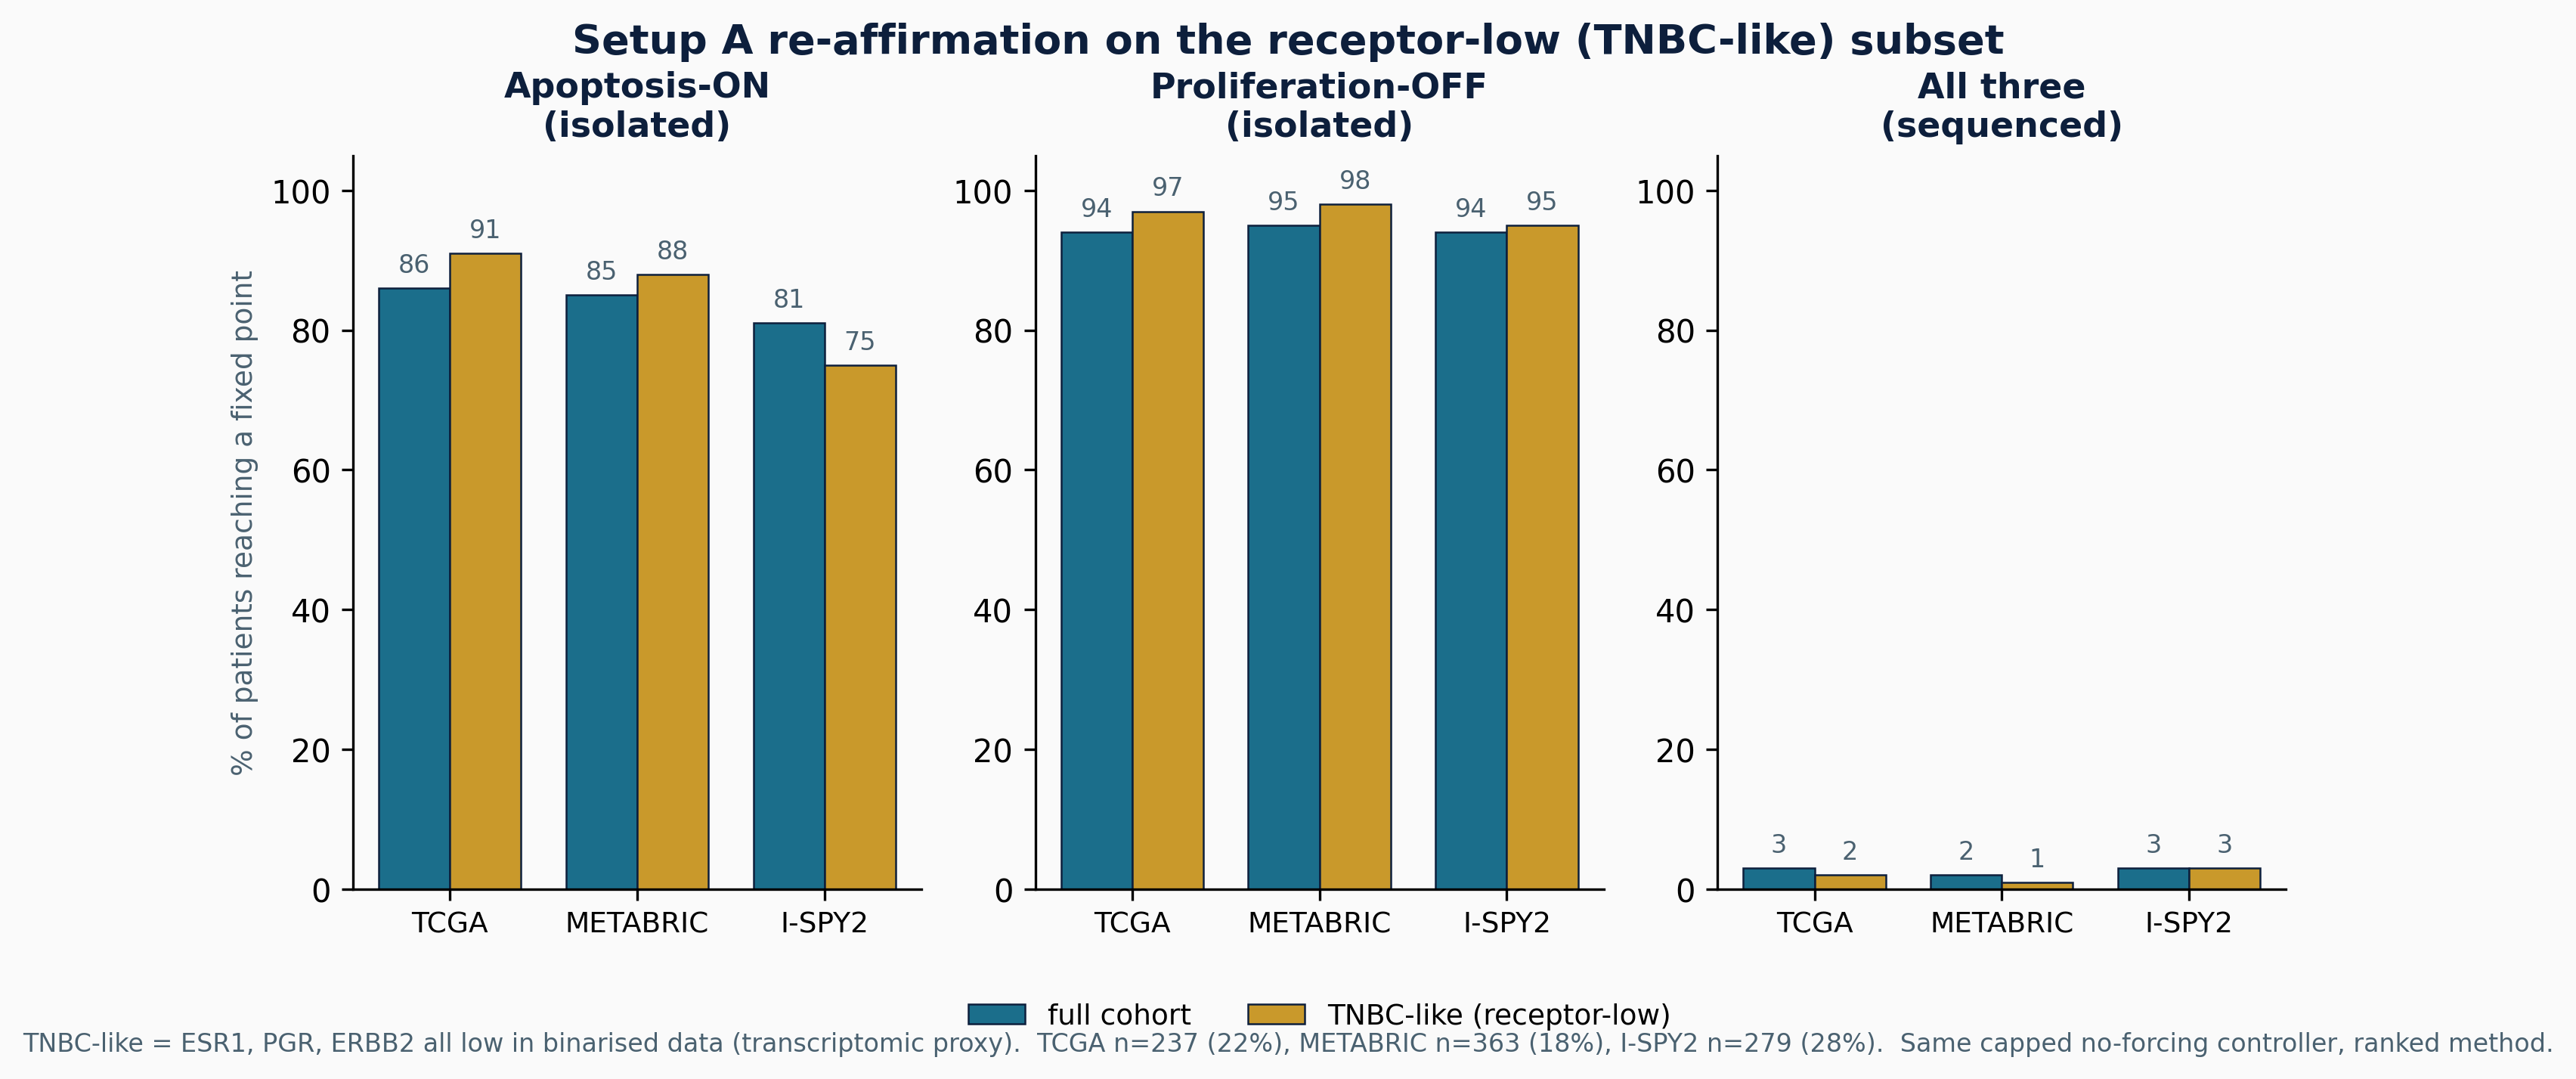
\includegraphics[width=\textwidth]{figures/figA_tnbc_panel.png}
\caption{\textbf{Re-affirmation on the receptor-low (TNBC-like) subset.} The Setup A static controller (ranked) on the full cohort (teal) and on the receptor-low subset (gold), the latter defined by low ESR1, PGR, and ERBB2 in the binarised data as a transcriptomic proxy for triple-negative status. Individual phenotypes remain highly controllable in the subset while the joint all-three rate stays in the low single digits, the same individual-versus-joint pattern as in the full cohort. Subset sizes: TCGA 237 (22\%), METABRIC 363 (18\%), I-SPY2 279 (28\%).}
\label{fig:tnbc}
\end{figure}

\subsection{The obstruction is a dominant strongly-connected core}
\label{sec:32}
The reason is structural. We build a directed coupling graph whose nodes are the 22 regulatory pathways, with an edge from one pathway to another when a node in the first appears in the update rule of the second, and we compute its strongly-connected components. A strongly-connected component is a set of pathways that all feed back into one another, so a signal injected anywhere in it can circulate to every member. The graph is dominated by one such component of 16 pathways, with a secondary component of two; together about 82\% of the regulatory pathways lie inside cyclic cores rather than in a clean feed-forward chain (Figure~\ref{fig:scc}).

The coupling is distributed, not funnelled through a single hub. The strongest carriers are AKT1, MAPK1, FOXO3, and TP53, but removing the AKT1 coupling shrinks the dominant component only from 16 pathways to 14, so no one or two ablations break the cycle. This is exactly the regime in which pathway-by-pathway stabilisation fails. Stabilising a pathway in isolation is sound only on a weakly coupled, acyclic network; inside a strongly-connected core the other members re-inject the very signals an intervention removes, so a phenotype can be feasible yet unreachable under any bounded, non-accumulating budget. This also locates the boundary of the earlier BBCN118 decomposition theorem, which holds under weak inter-pathway coupling: the full network does not meet that condition on the hard case, which is why the sequenced result collapses, and why the apoptosis core must be modelled on its own terms in Setup~B.

\begin{figure}[h]
\centering
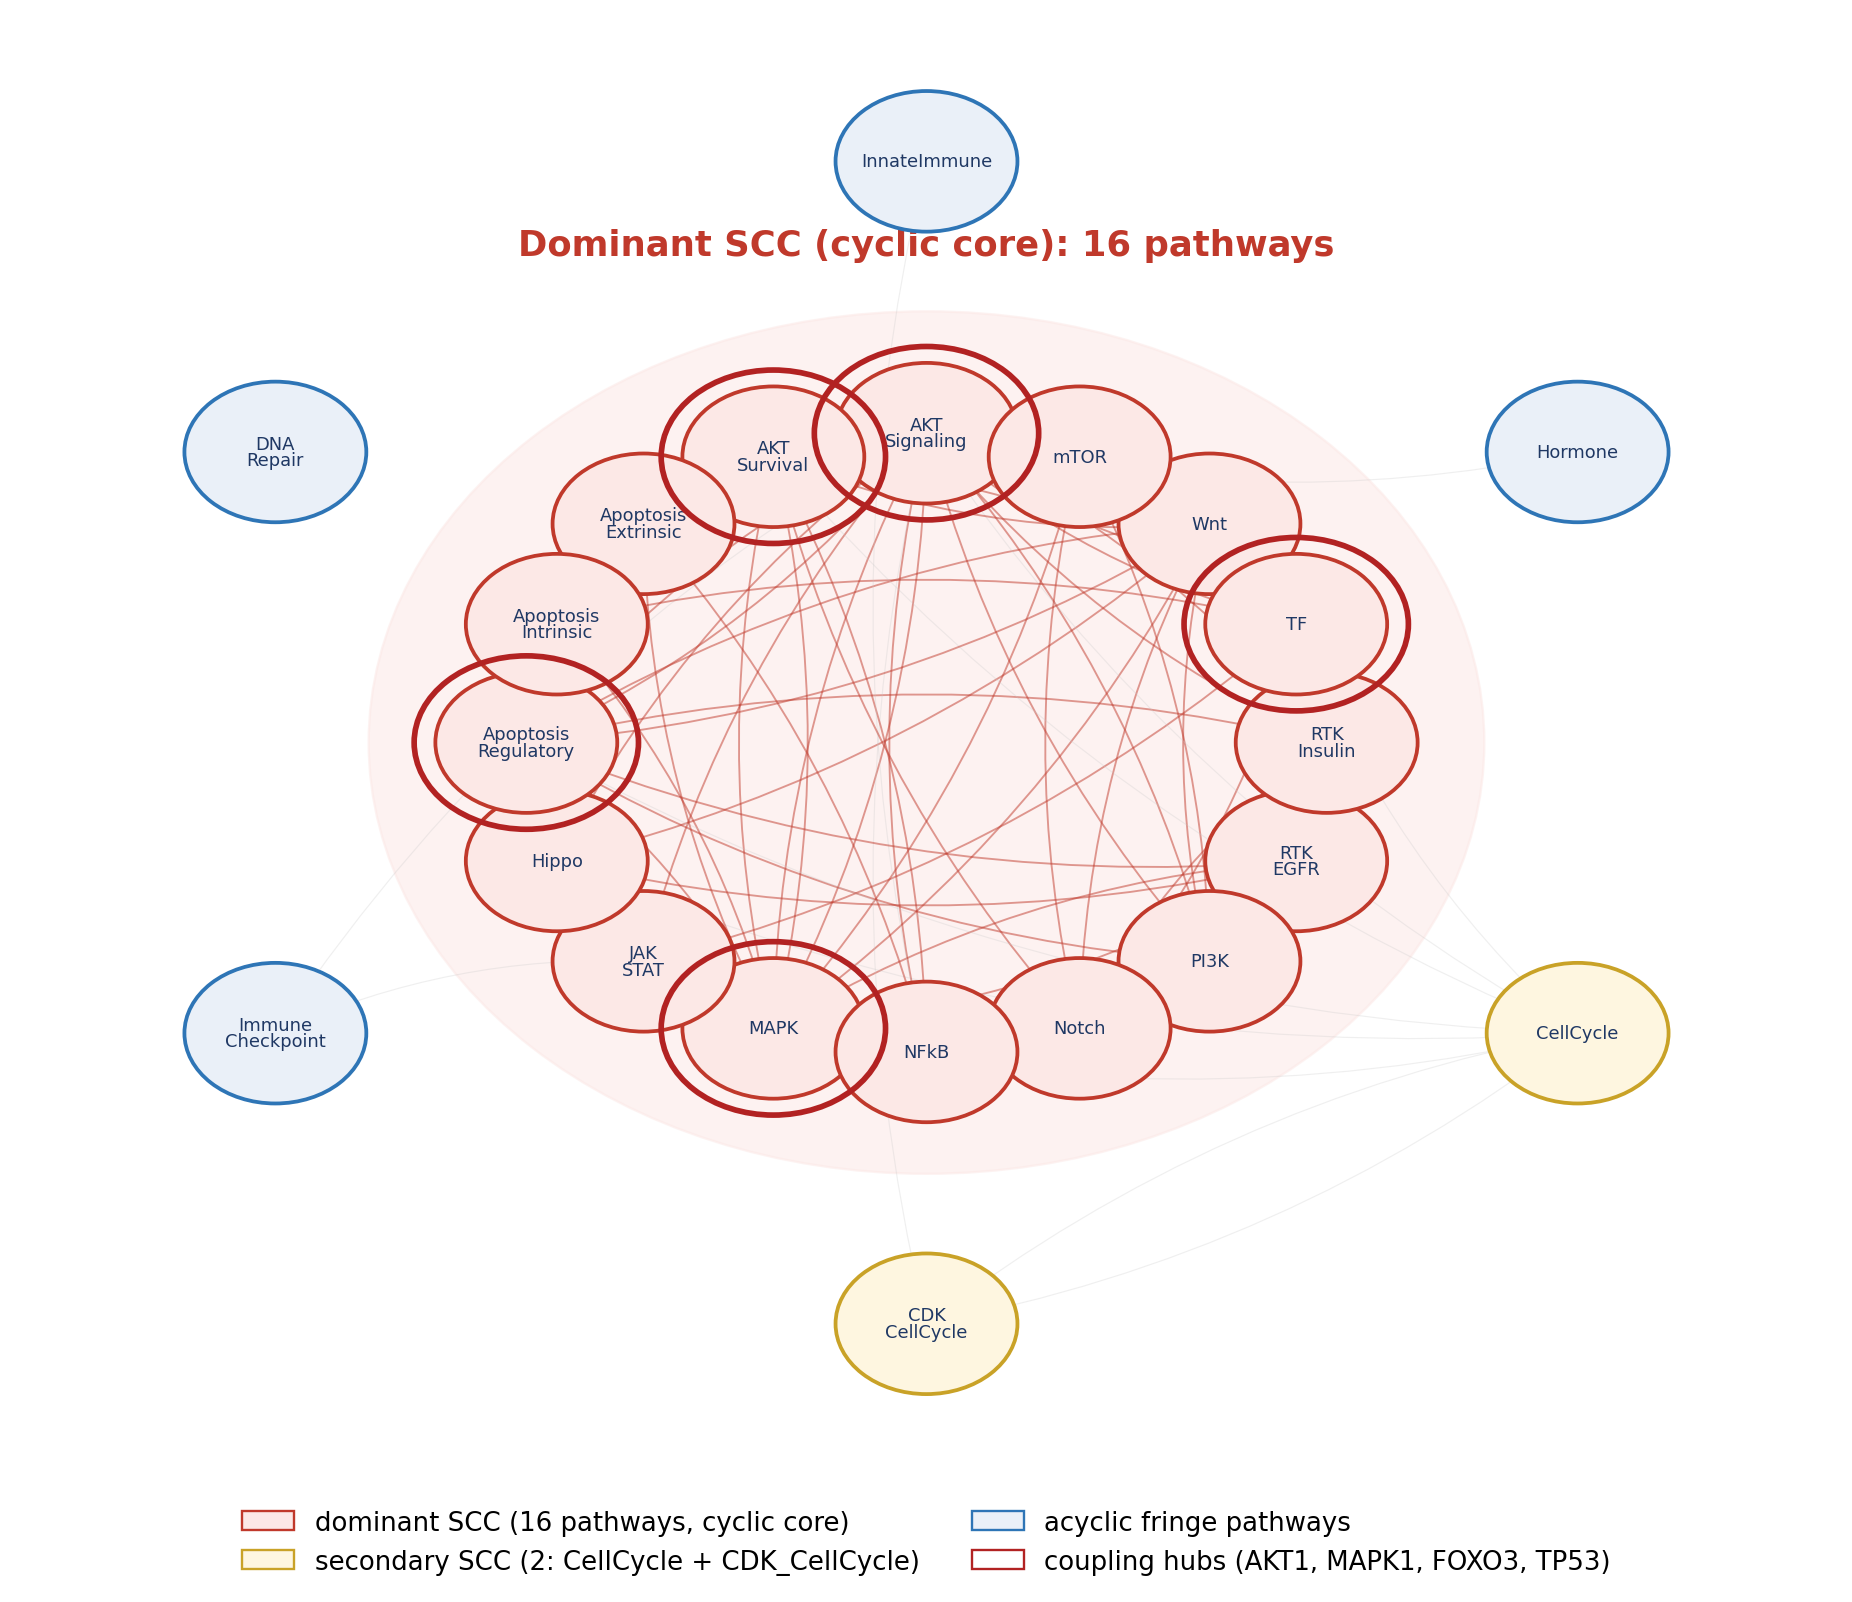
\includegraphics[width=0.6\textwidth]{figures/fig2_scc.png}
\caption{\textbf{The pathway coupling graph.} The dominant 16-pathway strongly-connected component is shaded as the cyclic core; the coupling hubs (AKT1, MAPK1, FOXO3, TP53) are ringed. The two auxiliary input modules are excluded.}
\label{fig:scc}
\end{figure}

\subsection{A bistable switch resolves the apoptosis core and routes patients coherently}
\label{sec:33}
Re-modelled as a bistable switch, the apoptosis core has two stable attractors: a survival state with AKT high and p53 low, and an apoptotic state with p53 high and AKT low. The control problem becomes flipping the switch rather than pushing a marker against the coupled core. Each patient's binarised state seeds the switch, which is run on the multirate schedule until it settles. Across the three cohorts the switch routes about half of patients to the apoptotic attractor (\BBCNBRoutingSwitchTcgaApopPct\%, \BBCNBRoutingSwitchMetabricApopPct\%, \BBCNBRoutingSwitchIspyTwoApopPct\% for TCGA, METABRIC, and I-SPY2), about a quarter to the survival attractor (\BBCNBRoutingSwitchTcgaSurvPct\%, \BBCNBRoutingSwitchMetabricSurvPct\%, \BBCNBRoutingSwitchIspyTwoSurvPct\%), and the remainder to a mixed outcome (Figure~\ref{fig:switch}, Table~\ref{tab:setupB}). The split is stable across the three platforms, so it is not a feature of one assay.

The routing is biologically coherent, which is what makes it more than a relabelling. Survival-routed patients are \BBCNBRoutingSwitchTcgaSurvUncoupledPct\%, \BBCNBRoutingSwitchMetabricSurvUncoupledPct\%, and \BBCNBRoutingSwitchIspyTwoSurvUncoupledPct\% in the uncoupled AKT--FOXO3a resistant state, against cohort-wide rates of \BBCNBRoutingSwitchTcgaUPct\%, \BBCNBRoutingSwitchMetabricUPct\%, and \BBCNBRoutingSwitchIspyTwoUPct\%, an enrichment of roughly threefold, and a multidrug-resistance signature is higher in the survival-routed group than in the apoptotic-routed group in every cohort. In other words, the switch sends precisely the biologically resistant patients to the survival attractor. That is a falsifiable prognostic alignment rather than an arbitrary partition: it states in advance which patients the model expects to resist apoptosis, and that prediction can be checked against independent resistance markers.

\begin{figure}[h]
\centering
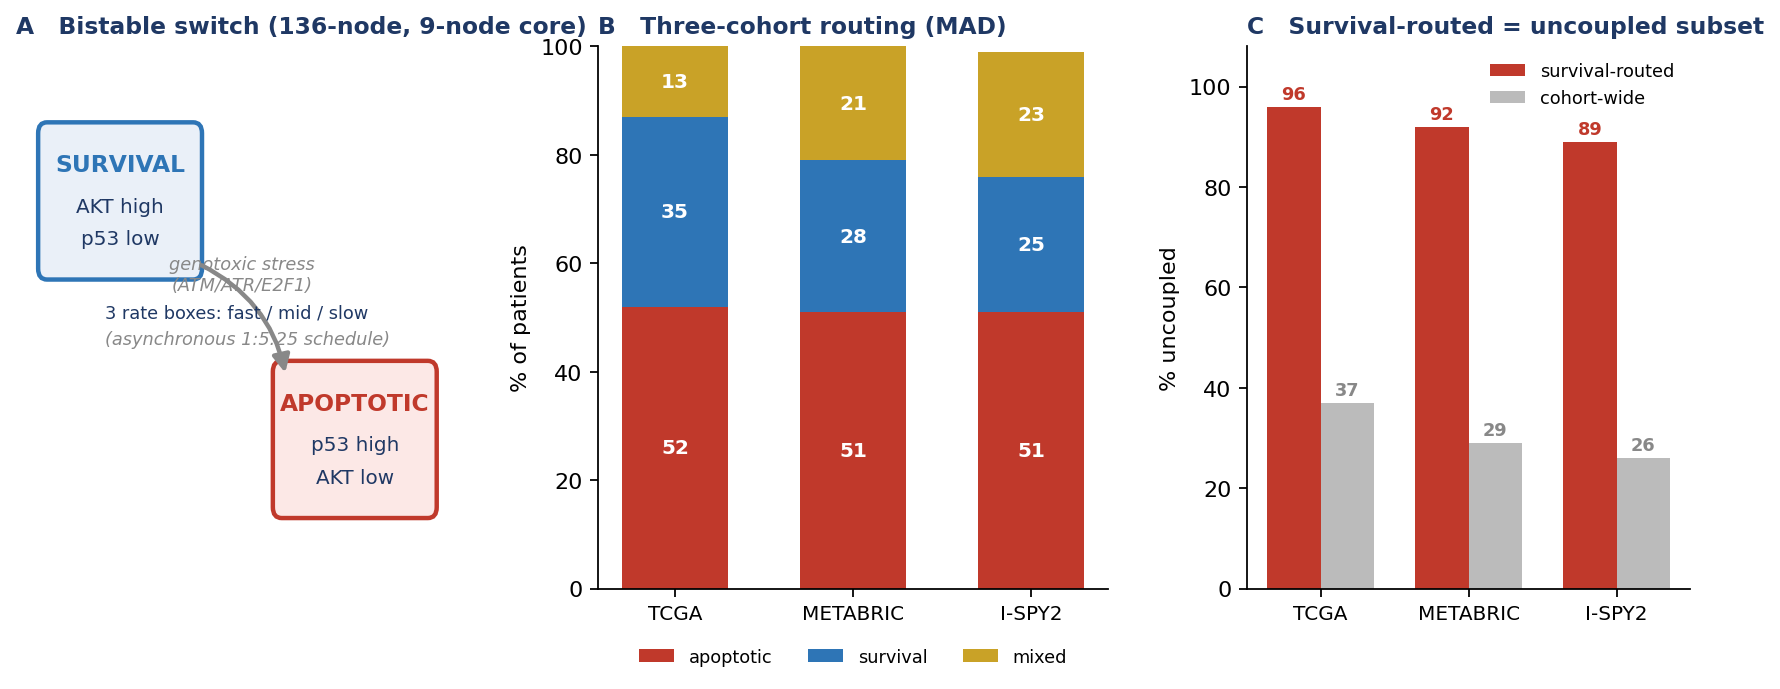
\includegraphics[width=\textwidth]{figures/figB.png}
\caption{\textbf{The bistable switch (136-node model).} (A) The two attractors and the survival$\to$apoptosis flip under sustained genotoxic stress. (B) Three-cohort routing (robust $z$-score): about half apoptotic, a quarter survival, the rest mixed, consistent across platforms. (C) Biological check: survival-routed patients are 89--95\% uncoupled, versus 26--37\% cohort-wide.}
\label{fig:switch}
\end{figure}

\begin{table}[h]
\centering
\caption{Setup~B switch routing and biological check (robust $z$-score, full cohorts).}
\label{tab:setupB}
\begin{tabular}{lcccc}
\toprule
Cohort ($N$) & Apoptotic & Survival & Mixed & SURV uncoupled \\
\midrule
TCGA (\BBCNBRoutingSwitchTcgaN)    & \BBCNBRoutingSwitchTcgaApopPct\% & \BBCNBRoutingSwitchTcgaSurvPct\% & \BBCNBRoutingSwitchTcgaMixedPct\% & \BBCNBRoutingSwitchTcgaSurvUncoupledPct\% vs \BBCNBRoutingSwitchTcgaUPct\% \\
METABRIC (\BBCNBRoutingSwitchMetabricN)& \BBCNBRoutingSwitchMetabricApopPct\% & \BBCNBRoutingSwitchMetabricSurvPct\% & \BBCNBRoutingSwitchMetabricMixedPct\% & \BBCNBRoutingSwitchMetabricSurvUncoupledPct\% vs \BBCNBRoutingSwitchMetabricUPct\% \\
I-SPY2 (\BBCNBRoutingSwitchIspyTwoN)   & \BBCNBRoutingSwitchIspyTwoApopPct\% & \BBCNBRoutingSwitchIspyTwoSurvPct\% & \BBCNBRoutingSwitchIspyTwoMixedPct\% & \BBCNBRoutingSwitchIspyTwoSurvUncoupledPct\% vs \BBCNBRoutingSwitchIspyTwoUPct\% \\
\bottomrule
\end{tabular}
\end{table}

\subsection{Residual resistance is a hysteresis property with a clear drug interpretation}
\label{sec:34}
The survival-routed patients are not rescued by survival-axis inhibition. Probing the settled switch directly, we find that inhibiting the survival inputs, the PI3K and RTK axis together with SRC, RHEB, and IGF1R, does not flip the resistant attractor to apoptosis. Only a genotoxic or oncogenic-stress input, modelled through ATM, ATR, and E2F1, flips it. This is hysteresis: once the uncoupled, self-sustaining survival state is established, withdrawing the upstream survival drive is not enough to cross back, because the apoptotic attractor is reachable only through the stress arm. Each timescale box is monostable on its own; the bistability, and therefore this resistance, is emergent from the coupling between boxes rather than present in any one of them.

The therapeutic reading is direct and splits the cohort in two. The flippable subset is addressable on the PI3K/AKT/mTOR axis, and the kernel designer concentrates on exactly that axis: PIK3CA is the leading actuator in every cohort, followed by AKT1 and the PDPK1/MTOR nodes, with the same ordering under both kernel methods (Figure~\ref{fig:kernelB}). The resistant subset is not budget-limited but mechanism-limited: it needs a genotoxic or stress-inducing agent, because survival-axis drugs alone cannot move it across the hysteresis barrier. This is a concrete, testable treatment hypothesis attached to a named patient stratum.

\begin{figure}[h]
\centering
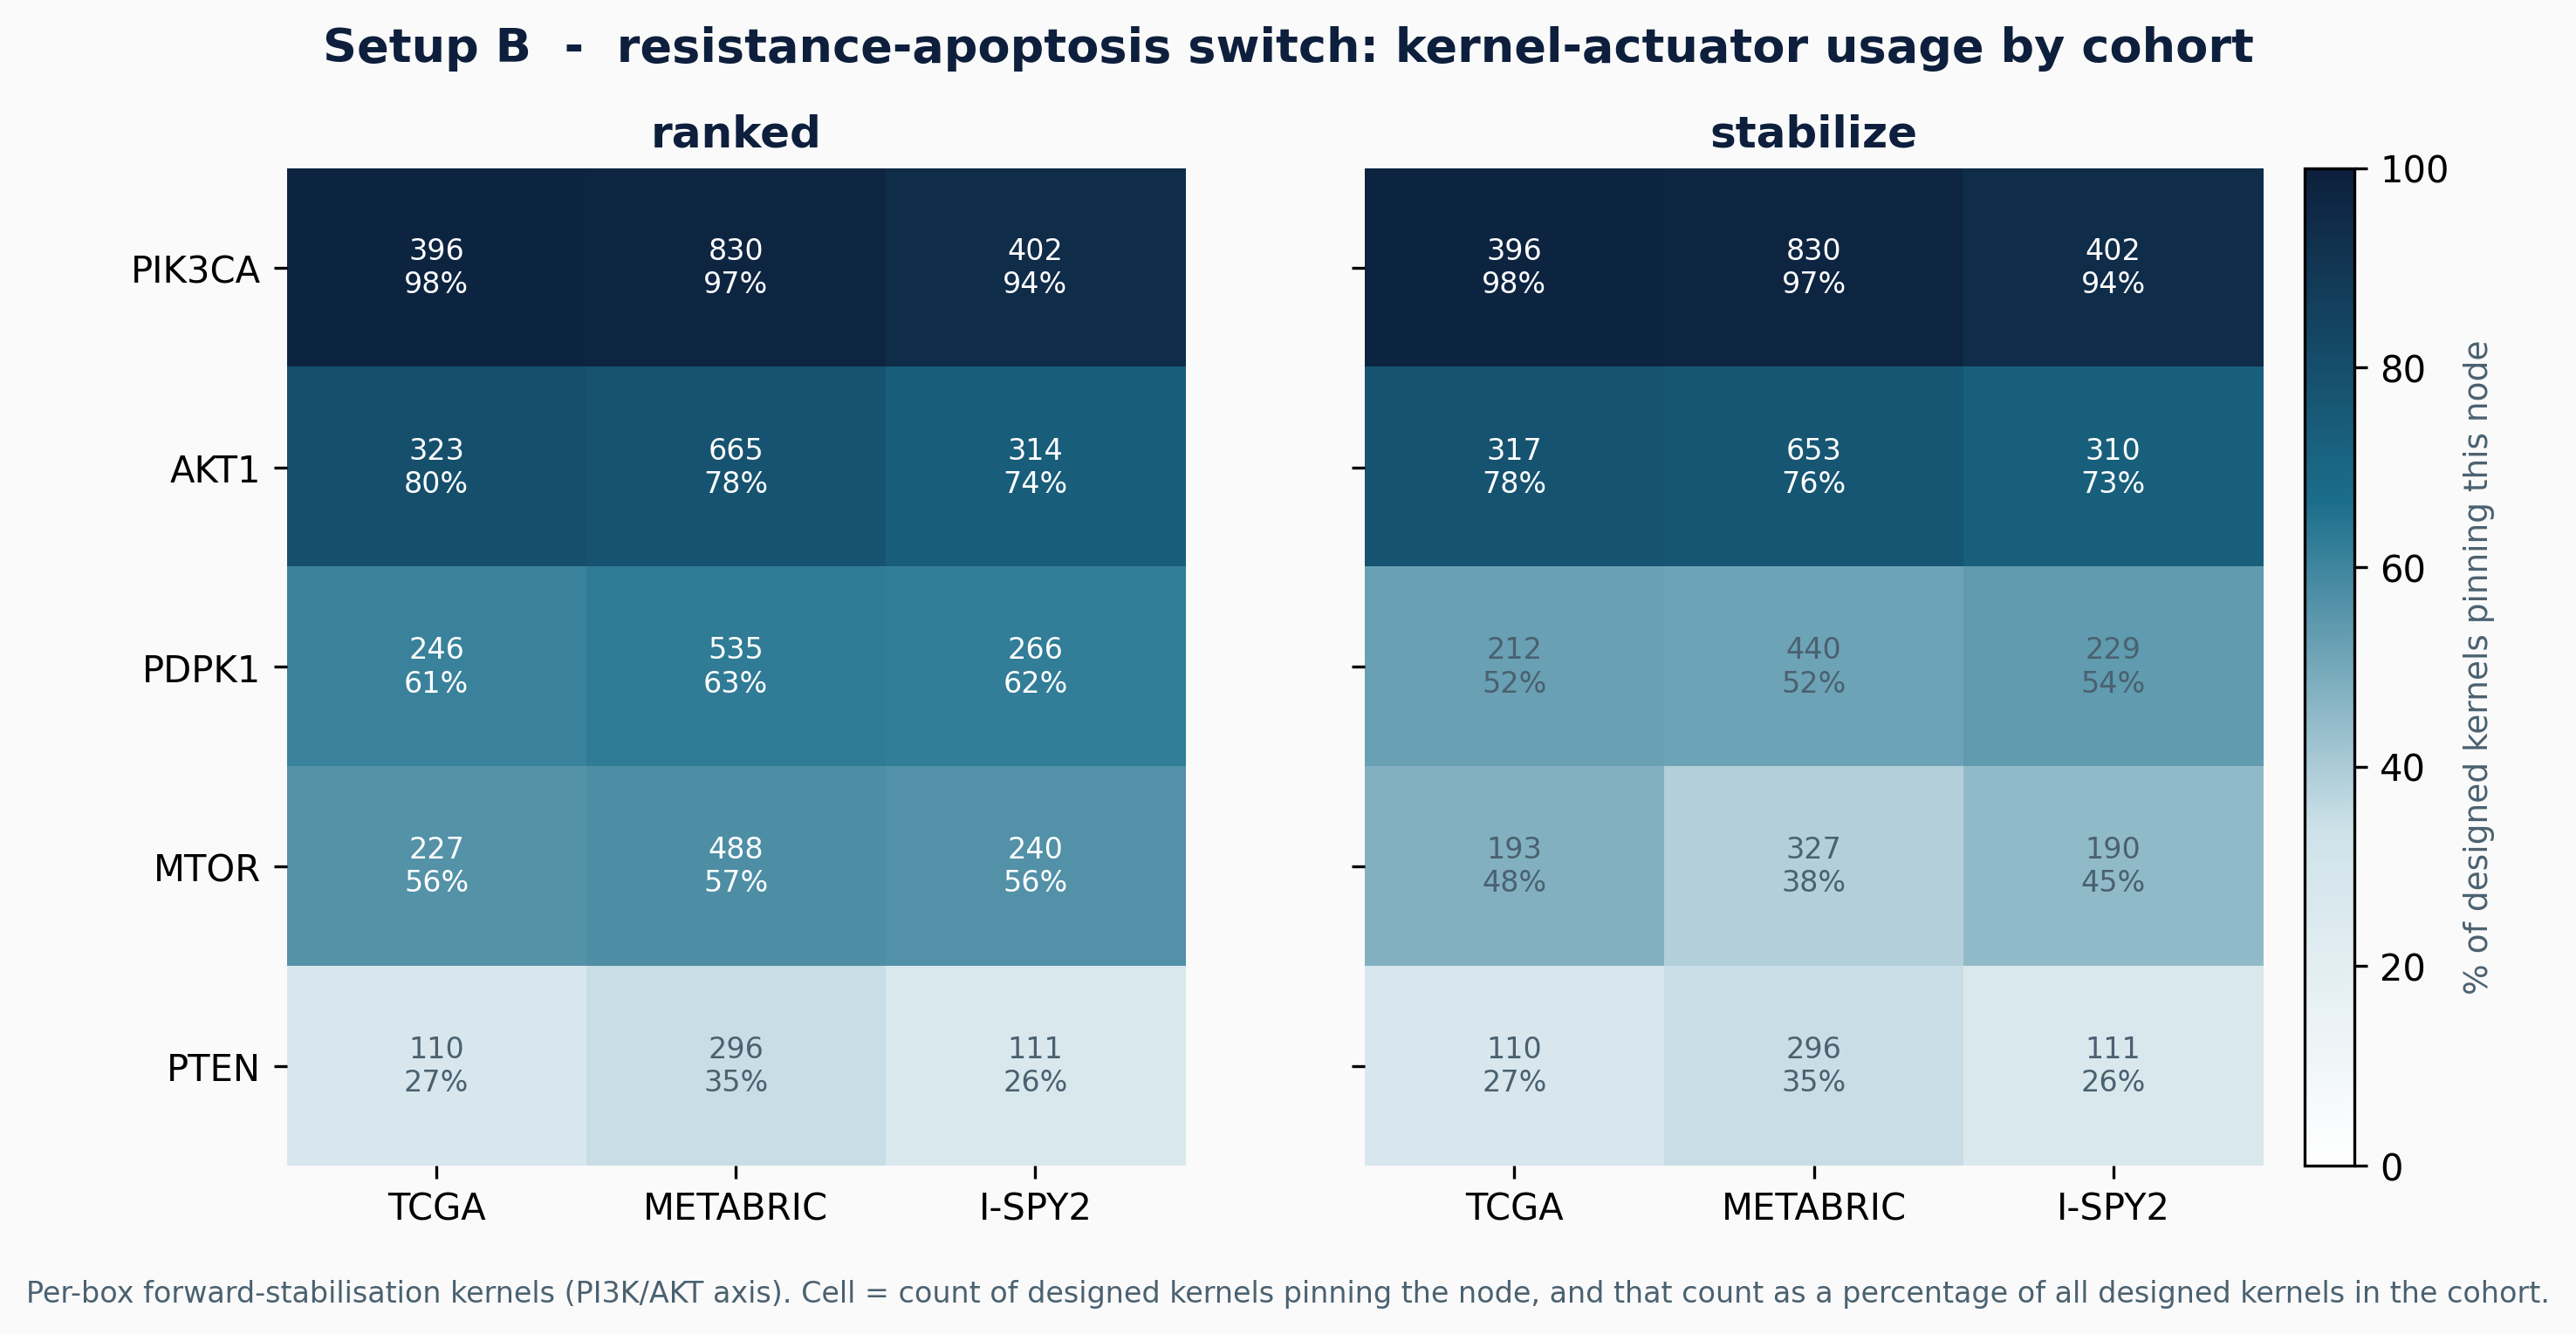
\includegraphics[width=\textwidth]{figures/figB_kernel_actuator.png}
\caption{\textbf{Setup~B kernel actuators: the PI3K/AKT/mTOR nomination.} For each cohort, the per-box forward-stabilisation kernels that flip resistant patients toward apoptosis are tallied by node, under the ranked heuristic (left) and the algebraic global-stabilisation test (right). Each cell gives the count of designed kernels that pin the node, and that count as a percentage of all designed kernels in the cohort. PIK3CA is pinned in almost every kernel (94--98\%), followed by AKT1 (73--80\%) and the PDPK1/MTOR nodes, with PTEN least used. The ordering is the same across all three cohorts and is essentially identical between the two methods, so the drug-target nomination is robust to both the cohort and the kernel-selection criterion. Counts are computed from the same pipeline that emits the flip rates of Table~\ref{tab:compare}.}
\label{fig:kernelB}
\end{figure}

This routing and its resistance signature are not an artefact of receptor-positive disease. On the same receptor-low (TNBC-like) subset, the switch routes patients in proportions close to the full cohort, and the survival-routed cells remain almost entirely in the uncoupled resistant state (Figure~\ref{fig:tnbcB}). The hysteresis reading of residual resistance therefore holds across receptor subtypes.

\begin{figure}[h]
\centering
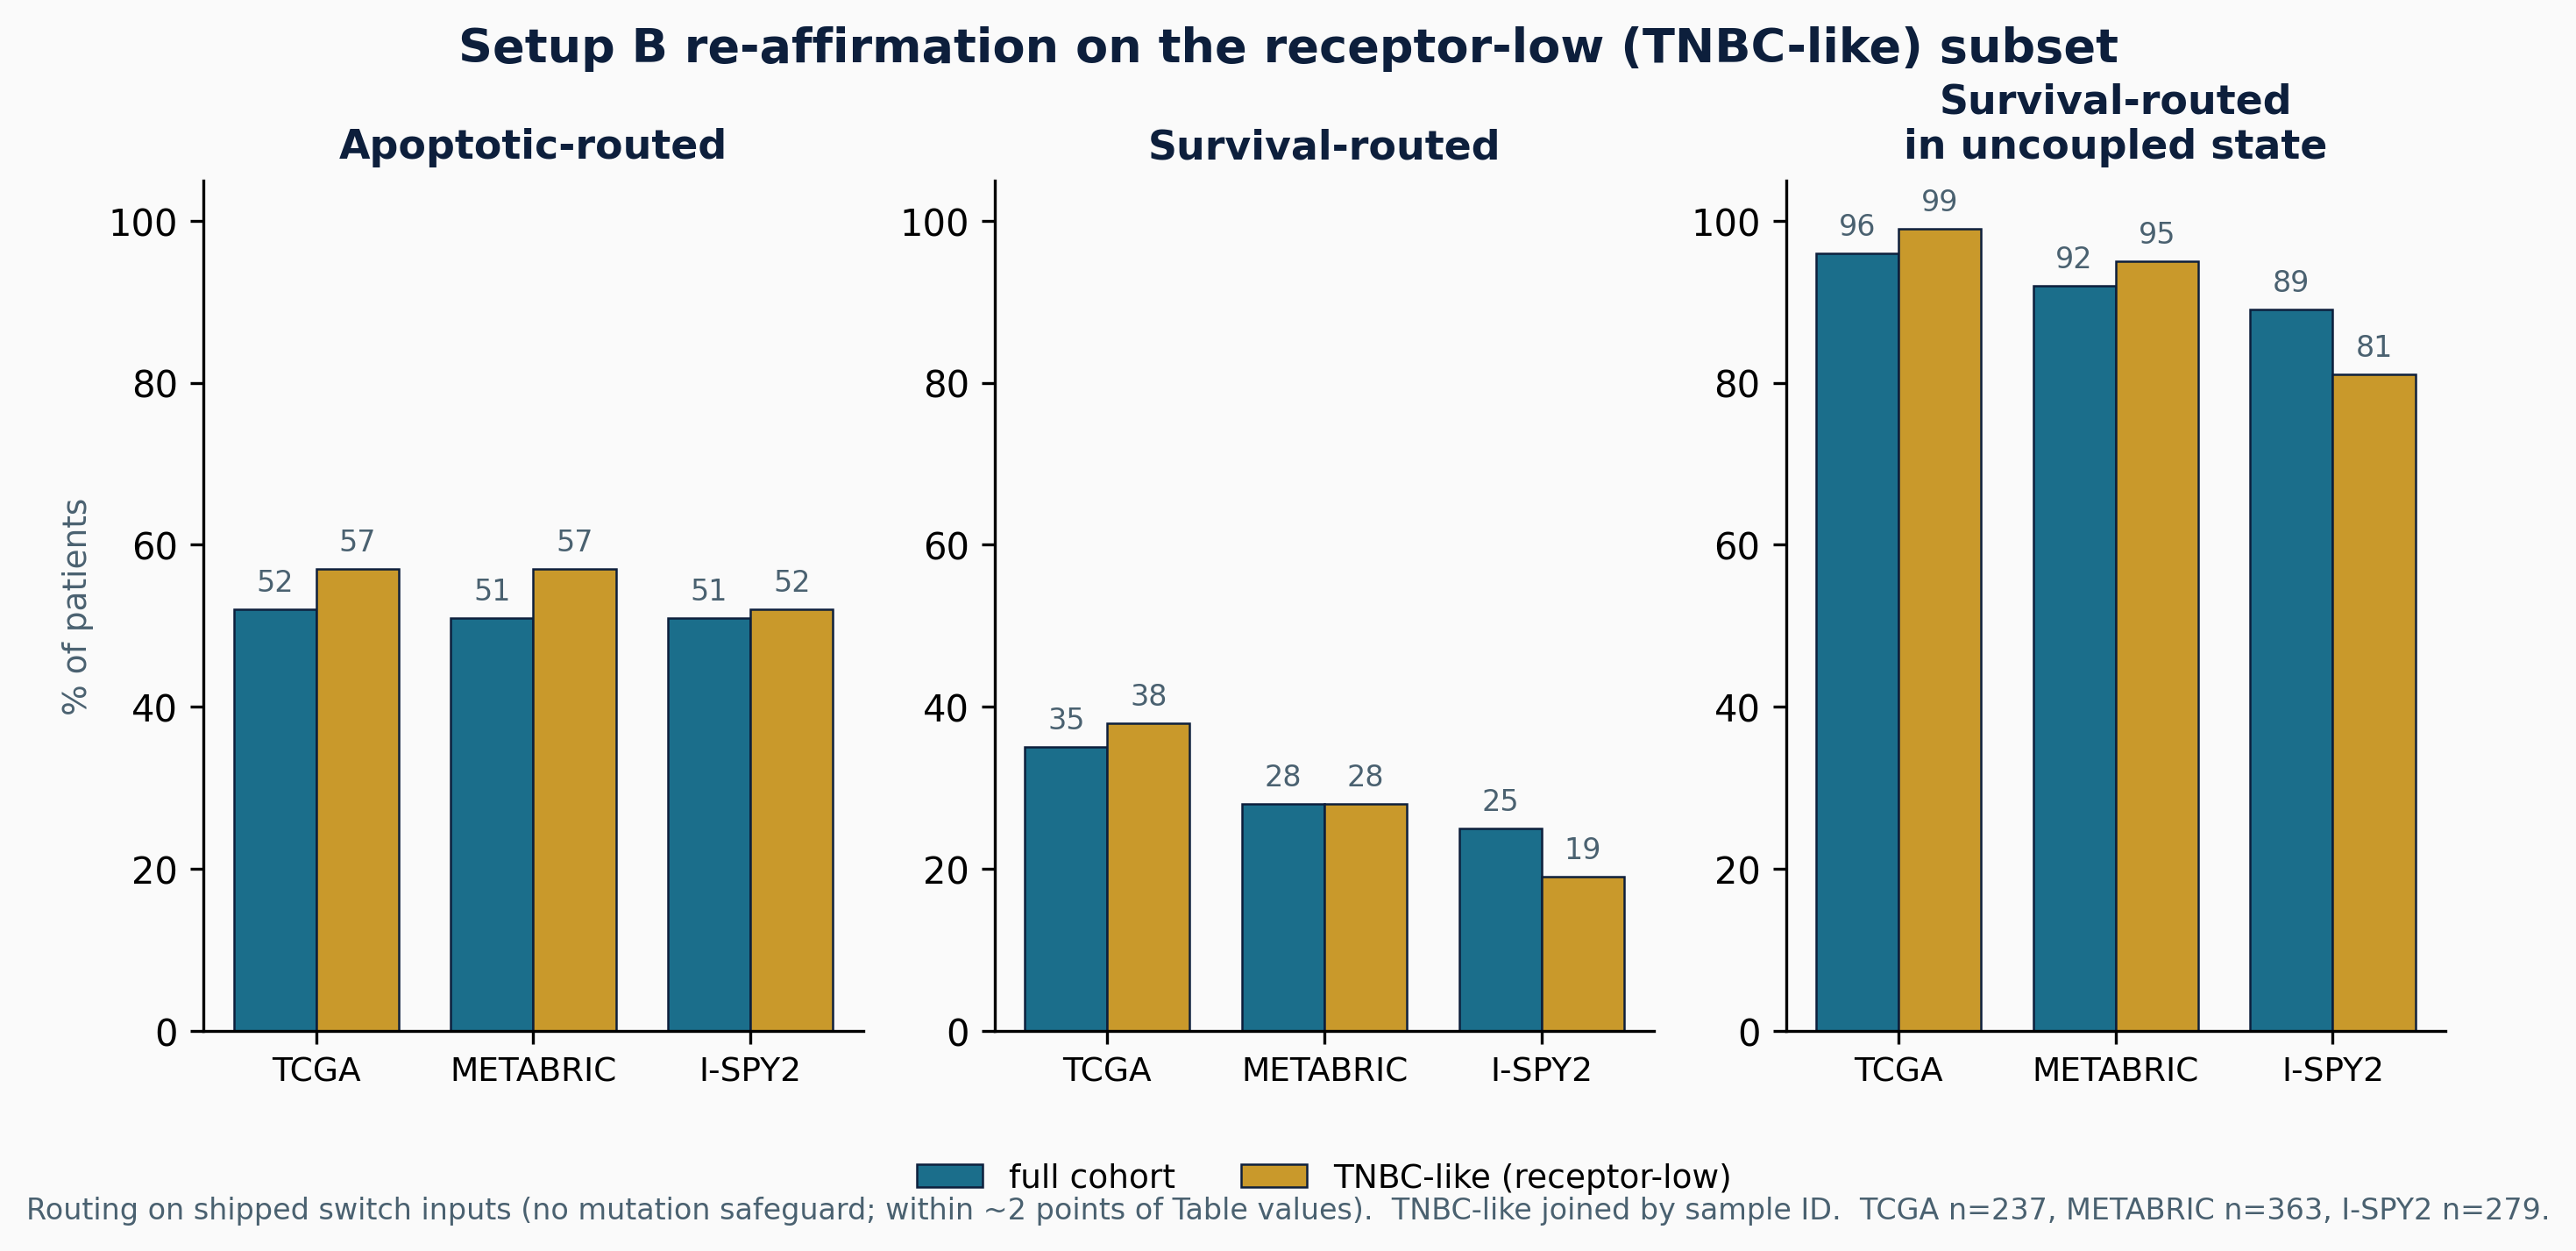
\includegraphics[width=\textwidth]{figures/figB_tnbc_panel.png}
\caption{\textbf{Setup B routing re-affirmed on the receptor-low (TNBC-like) subset.} Switch routing (apoptotic, survival) and the survival-routed uncoupled rate, for the full cohort (teal) and the receptor-low subset (gold). Routing here is computed on the shipped switch inputs without the mutation safeguard, so the percentages sit within about two points of the Table~\ref{tab:setupB} values; the within-cohort full-versus-subset comparison uses the same method throughout. The survival-routed uncoupled enrichment, which is the structural basis of the hysteresis reading, holds in the subset.}
\label{fig:tnbcB}
\end{figure}

\subsection{Validation, and the limits of prediction}
\label{sec:35}
The nominated targets are real: the kernel genes (PIK3CA, AKT1, MTOR) are established, mostly-approved breast-cancer drug targets in curated drug-target evidence, and this concordance is robust across all three input front-ends (median-binarised expression, multi-gene signatures, and phospho-protein activity). Mutation concordance is weaker (METABRIC $p\approx0.02$; TCGA not significant), as expected when the model reads pathway activity rather than genotype. The model does not predict pathologic complete response: on the I-SPY2 AKT-inhibitor arm the routing is not concordant with pCR, and we ruled out two explanations, binarisation (continuous and binarised inputs are equally flat) and expression-versus-signalling (phospho-seeded inputs fail at pCR too). The remaining explanation is endpoint distance: pCR is a distal, whole-tumour outcome shaped by immune, stromal, and pharmacokinetic factors beyond the single-cell decision the switch models. The defensible role of the model is a structural stratifier and drug-target nominator, not a response predictor.
\authornote{survival-association and cell-line concordance to be reconciled to the current model version before inclusion; the public-repo position is an explicit null on survival benefit, stated honestly.}

\subsection{The two kernel methods, and the static and dynamic controllers, compared}
\label{sec:comparison}
Both kernel designs, the ranked reachability heuristic and the algebraic global-stabilisation test (Section~\ref{sec:methodsB}, Tier~1), were run on both the static controller (which fixes the per-phenotype pathway set) and the dynamic CDE controller (which selects pathways by failure classification), on all three cohorts at full $N$. Table~\ref{tab:compare} reports the per-phenotype results; routing in Setup~B is unaffected by the kernel method, since kernels are designed only after a patient is routed.

Three readings follow. First, the ranked method reproduces the earlier BBCN118 kernels exactly, so the heuristic results are preserved rather than discarded. Second, on the static controller the two methods are close (apoptosis differs by at most a few points), because for the per-pathway targets used here the patient's own state already lies in the stabilising basin. Third, on the dynamic controller the algebraic method certifies fewer passes than the heuristic, the gap being largest on proliferation (TCGA \BBCNACdeRankedTcgaStagepassProliferationOff\% ranked versus \BBCNACdeStabilizeTcgaStagepassProliferationOff\% algebraic), because it demands that the clamp drive \emph{every} pathway state to target, not only the patient's starting state. The algebraic figure is the conservative, provable one; the difference between the two columns is exactly the set of patients the heuristic counts from a favourable initial state that are not globally stabilisable. In Setup~B the two methods give identical flip rates in every cohort (TCGA \BBCNBKernelRankedTcgaFlipPct\% vs \BBCNBKernelStabilizeTcgaFlipPct\%, METABRIC \BBCNBKernelRankedMetabricFlipPct\% vs \BBCNBKernelStabilizeMetabricFlipPct\%, I-SPY2 \BBCNBKernelRankedIspyTwoFlipPct\% vs \BBCNBKernelStabilizeIspyTwoFlipPct\%), with PIK3CA the leading actuator throughout: on the small bistable boxes the algebraic test confirms the heuristic kernel rather than contradicting it.

Beyond the pass rates, the kernels themselves have a clear and interpretable structure. Across all three cohorts the controller leans on a compact, stable set of actuators: PTEN, SOS1, NOS3, and GRB2 are selected for essentially every patient, with the next tier drawn from the RTK, MAPK, and PI3K hubs (Figure~\ref{fig:kernelAusage}). The two methods agree on this dominant set but differ at the margin in a revealing way. The algebraic test drops MAP2K1 entirely while raising EGF and INS to universal use, and it trims the redundant ABL1 and PIK3CA selections, because it keeps only nodes that drive every pathway state to target rather than the patient's state alone. Mapping each kernel to the pathway it serves shows a near block-diagonal pattern (Figure~\ref{fig:kernelAblock}): each actuator acts within its own pathway module, with little off-diagonal leakage. Control is therefore sparse and pathway-localised, which is what makes the kernels interpretable as drug targets. This is not in tension with the strong-coupling obstruction of Section~\ref{sec:32}. The place where control is \emph{applied} is modular, but the free dynamics still carry its effects around the cyclic core, which is why local application does not translate into joint reachability.

\begin{figure}[h]
\centering
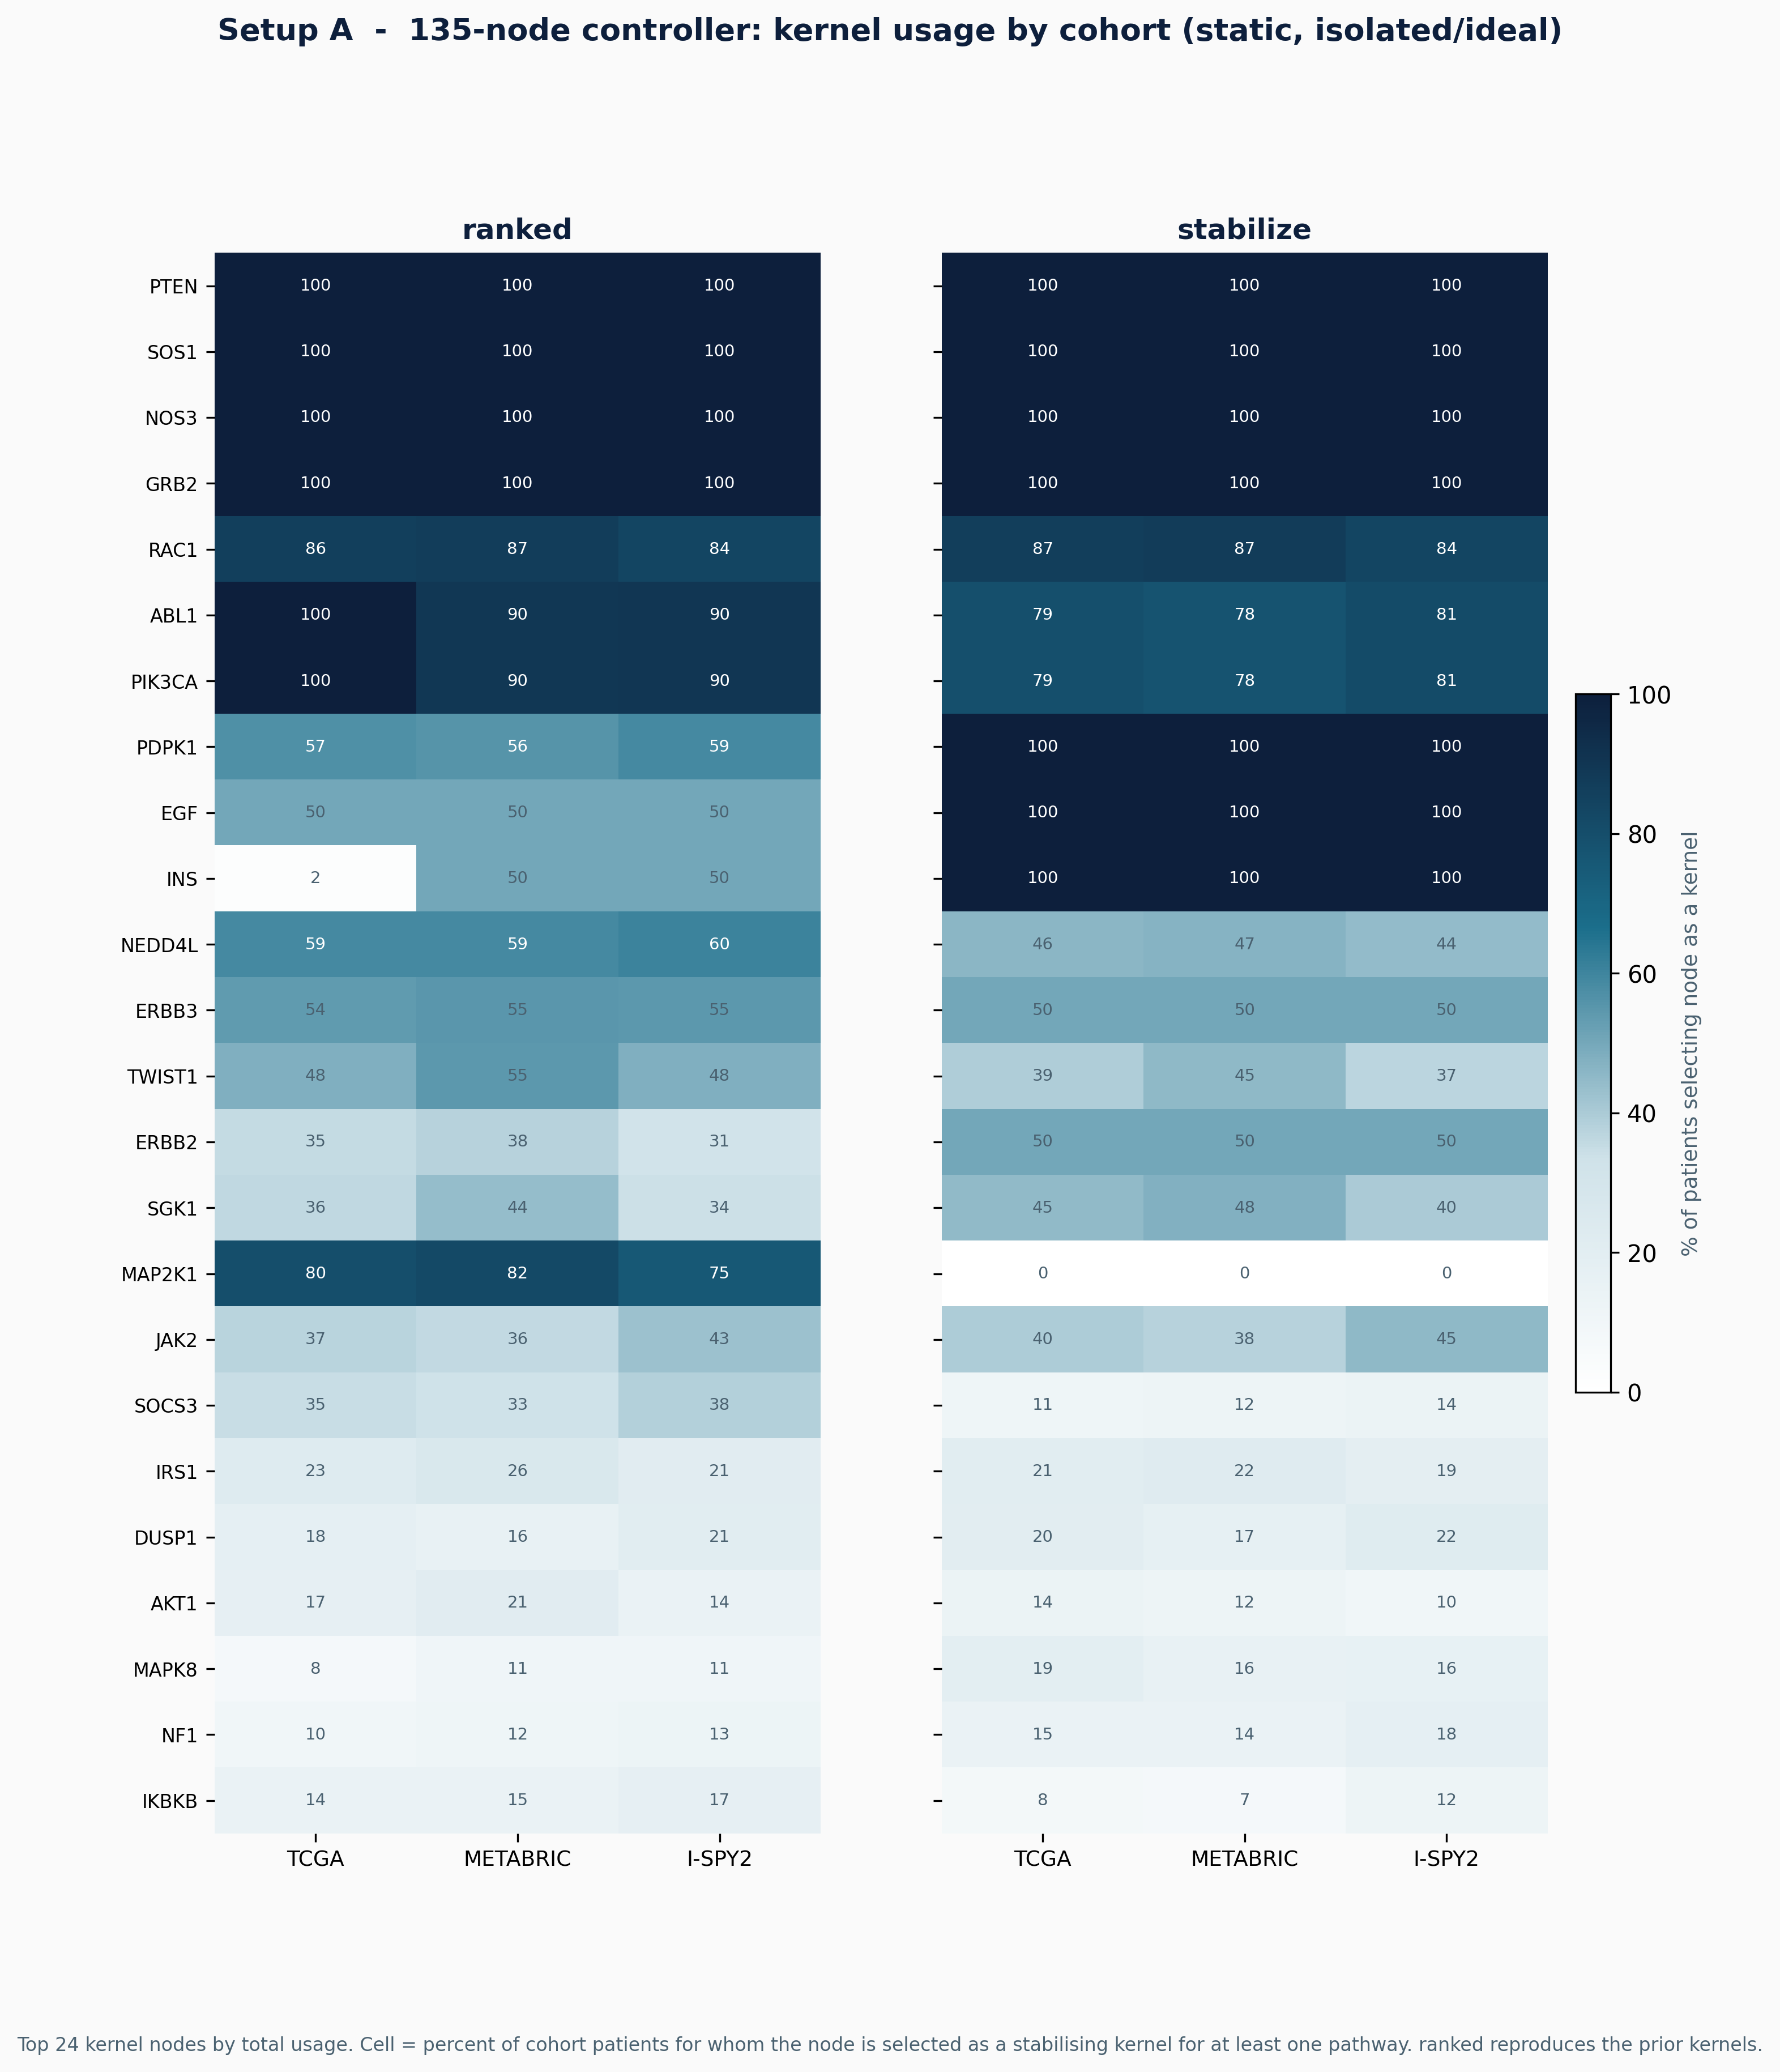
\includegraphics[width=\textwidth]{figures/figA_kernel_usage.png}
\caption{\textbf{Setup~A kernel usage by cohort.} The 24 most-used kernel nodes under the static, isolated/ideal controller, shown for the ranked heuristic (left) and the algebraic test (right); each cell is the percentage of cohort patients for whom the node is selected as a stabilising kernel for at least one pathway. A small core, PTEN, SOS1, NOS3, and GRB2, is used for every patient in every cohort. The method contrast is informative: the algebraic test sets MAP2K1 to zero and EGF and INS to full use, reflecting its stricter global-stabilisation criterion, while the dominant nodes are unchanged. The usage pattern is stable across TCGA, METABRIC, and I-SPY2.}
\label{fig:kernelAusage}
\end{figure}

\begin{figure}[h]
\centering
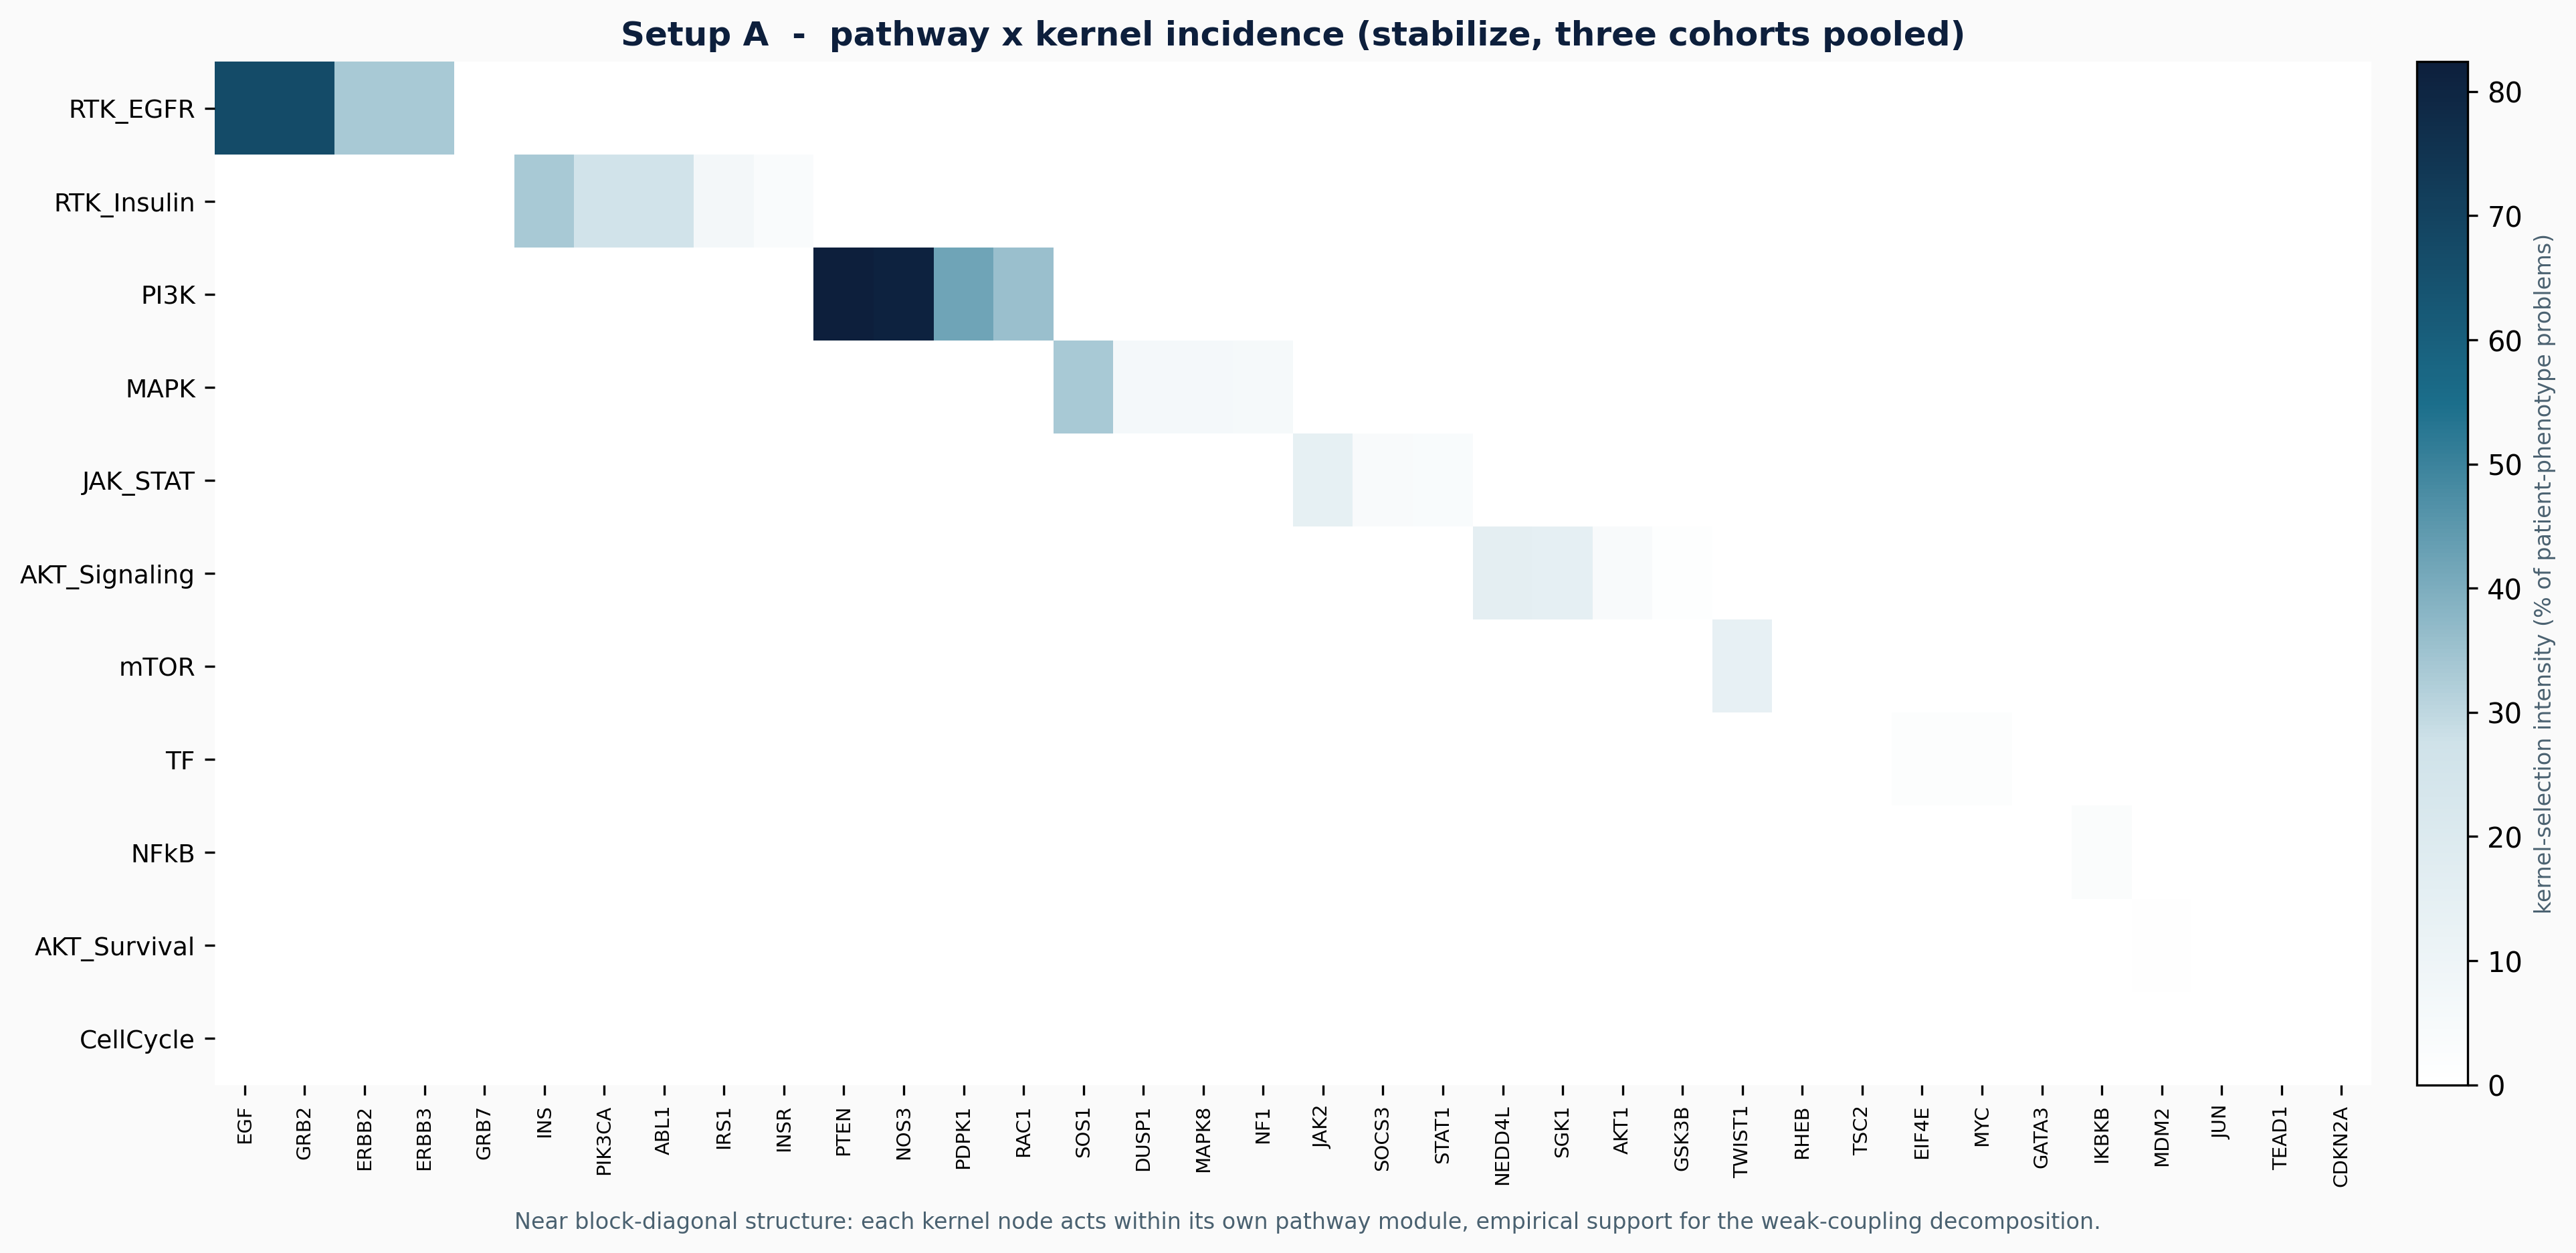
\includegraphics[width=\textwidth]{figures/figA_pathway_kernel.png}
\caption{\textbf{Setup~A pathway-by-kernel incidence: control is modular.} Kernel-selection intensity for each pathway and node pair, pooled over the three cohorts under the algebraic test. The near block-diagonal structure shows that each kernel node acts inside its own pathway module: RTK kernels on EGF, GRB2, and ERBB2; the PI3K kernel on PTEN, NOS3, and PDPK1; MAPK on SOS1, DUSP1, and NF1; JAK--STAT on JAK2 and SOCS3; AKT on NEDD4L, SGK1, and AKT1; and mTOR on TWIST1 and RHEB. Interventions are sparse and pathway-confined; their effects nonetheless propagate through the coupled core of Figure~\ref{fig:scc}, which is why modular application does not yield joint reachability.}
\label{fig:kernelAblock}
\end{figure}

\begin{table}[h]
\centering
\caption{Kernel-method and controller comparison (\% reaching target), full cohorts. Static = fixed pathway set; CDE = dynamic failure-classification selection. Each cell pair is ranked\,$\vert$\,algebraic.}
\label{tab:compare}
\begin{tabular}{llcccc}
\toprule
& & \multicolumn{2}{c}{Static controller} & \multicolumn{2}{c}{Dynamic CDE} \\
\cmidrule(lr){3-4}\cmidrule(lr){5-6}
Cohort & Phenotype & ranked & algebraic & ranked & algebraic \\
\midrule
TCGA     & Apoptosis      & \BBCNAStaticRankedTcgaIsoApoptosisOn & \BBCNAStaticStabilizeTcgaIsoApoptosisOn & \BBCNACdeRankedTcgaStagepassApoptosisOn & \BBCNACdeStabilizeTcgaStagepassApoptosisOn \\
         & Proliferation  & \BBCNAStaticRankedTcgaIsoProliferationOff & \BBCNAStaticStabilizeTcgaIsoProliferationOff & \BBCNACdeRankedTcgaStagepassProliferationOff & \BBCNACdeStabilizeTcgaStagepassProliferationOff \\
METABRIC & Apoptosis      & \BBCNAStaticRankedMetabricIsoApoptosisOn & \BBCNAStaticStabilizeMetabricIsoApoptosisOn & \BBCNACdeRankedMetabricStagepassApoptosisOn & \BBCNACdeStabilizeMetabricStagepassApoptosisOn \\
         & Proliferation  & \BBCNAStaticRankedMetabricIsoProliferationOff & \BBCNAStaticStabilizeMetabricIsoProliferationOff & \BBCNACdeRankedMetabricStagepassProliferationOff & \BBCNACdeStabilizeMetabricStagepassProliferationOff \\
I-SPY2   & Apoptosis      & \BBCNAStaticRankedIspyTwoIsoApoptosisOn & \BBCNAStaticStabilizeIspyTwoIsoApoptosisOn & \BBCNACdeRankedIspyTwoStagepassApoptosisOn & \BBCNACdeStabilizeIspyTwoStagepassApoptosisOn \\
         & Proliferation  & \BBCNAStaticRankedIspyTwoIsoProliferationOff & \BBCNAStaticStabilizeIspyTwoIsoProliferationOff & \BBCNACdeRankedIspyTwoStagepassProliferationOff & \BBCNACdeStabilizeIspyTwoStagepassProliferationOff \\
\bottomrule
\end{tabular}
\end{table}

% ------------------------------------------------------------
\section{Discussion}
Two findings carry the work. First, cell-fate phenotypes in this network are individually controllable but jointly near-exclusive, because they share a dominant strongly-connected core; feasibility does not imply reachability, and pathway-by-pathway control fails on the core. This complements stable-motif and STP control theory, which establish when a target attractor is controllable, by showing that under a realistic capped budget on real patient states the binding constraint is joint reachability across coupled phenotypes. Second, the hardest phenotype is best understood not as a target to push but as one attractor of a bistable resistance--apoptosis switch, and flipping it requires crossing a hysteresis barrier that survival-axis inhibition alone cannot cross. Embedding biological timescale separation as a Boolean-ARMA / multirate structure is what makes the core controllable where the whole-network controller could not.

The validated outputs are a coherent patient stratification and a robust PI3K/AKT/mTOR drug-target nomination independent of input front-end. The honest limit is that the model does not predict pathologic complete response, which we attribute to endpoint distance rather than signal quality. The framework is a mechanistic hypothesis generator and structural stratifier; clinical benefit is not demonstrated here.
\authornote{limitations (proxy $U$ flag; invasion out of scope; primary tumours only; binary modelling choice) and the road to clinical testing to be expanded at prose stage.}

% ------------------------------------------------------------
\section*{Code and data availability}
All numbers, figures, and tables regenerate from the companion repository
(\url{https://github.com/AamerIqbalBhatti/Systems-Biology-Journal-2026}) with a single command (\texttt{python reproduce\_all.py}); both setups run from
small shipped CSV files (a few hundred KB per cohort), so no large downloads are required. One-click
reproduction is also provided via Google Colab and Binder.

% ------------------------------------------------------------
\appendix
% AUTO-GENERATED by generate_rules_appendix.py from setup_a/bbcn/pathways.py -- DO NOT EDIT BY HAND.
\section{The BBCN digital logic model}
\label{app:rules}
This appendix lists the complete Boolean update logic of the BBCN network, one block per pathway module, generated directly from the source file \texttt{pathways.py} so that the printed rules cannot drift from the code. For each node, the right-hand side is its update rule over intra-pathway nodes and external bus inputs; \texttt{AND}, \texttt{OR}, \texttt{NOT} are the Boolean connectives. A node with rule equal to a single input is a pass-through of that input.

\paragraph{RTK EGFR. (Upstream\_RTK)}\mbox{}\\
\begin{flushleft}\ttfamily\small
EGF = EGF\\
EGFR = (EGF OR (ERBB2 AND ERBB3)) AND NOT MAP2K1\\
GRB2 = IRS1 OR (LATS1 OR (EGFR OR SRC))\\
GRB7 = GRB7 AND NOT PRKACA\\
ERBB2 = ERBB3 OR EGF\\
ERBB3 = NRG1 OR ERBB2\\
\end{flushleft}

\paragraph{RTK INSULIN. (Upstream\_RTK)}\mbox{}\\
\begin{flushleft}\ttfamily\small
INS = INS\\
INSR = INS OR FOXO3\\
IRS1 = NOT RPS6KB1 AND (INSR OR IGF1R)\\
PIK3CA = GRB2 OR IRS1\\
ABL1 = GRB2 OR EGFR OR ERBB2 OR IRS1\\
\end{flushleft}

\paragraph{HORMONE. (Upstream\_Hormone)}\mbox{}\\
\begin{flushleft}\ttfamily\small
AR = FOXO3 OR NOT AKT1\\
PGR = ESR1\\
ESR1 = (FOXO3 OR KMT2D) AND NOT AKT1\\
KMT2D = PAX7\\
\end{flushleft}

\paragraph{PI3K. (Terminal\_support)}\mbox{}\\
\begin{flushleft}\ttfamily\small
PTEN = NOT SRC\\
PDPK1 = (PIK3CA AND NOT PTEN) OR IGF1R\\
RAC1 = (PIK3CA OR DVL1) AND NOT AKT1\\
NOS3 = HSP90AA1 OR AKT1\\
\end{flushleft}

\paragraph{MAPK. (Resistance)}\mbox{}\\
\begin{flushleft}\ttfamily\small
HRAS = SOS1 AND NOT NF1\\
MAP2K1 = RAF1\\
RAF1 = HRAS OR KRAS\\
KRAS = SOS1\\
SOS1 = GRB2\\
NF1 = (TP53 OR FOXO3) AND NOT (MAPK1 OR AKT1)\\
MAPK8 = (FAS OR TRADD) AND NOT (AKT1 OR MAPK1)\\
MAPK1 = MAP2K1 AND NOT DUSP1\\
DUSP1 = MAPK1 OR MAPK8 OR JUN\\
\end{flushleft}

\paragraph{WNT. (Invasion\_OFF)}\mbox{}\\
\begin{flushleft}\ttfamily\small
APC = AXIN1\\
AXIN1 = NOT DVL1 AND GSK3B\\
CTNNB1 = NOT (APC AND AXIN1 AND GSK3B) AND (WNT1 OR SRC OR YAP1)\\
DVL1 = FZD3 OR NF1\\
FZD3 = WNT1 OR CREB1\\
RND1 = GRB7 OR DVL1\\
TCF7L2 = CTNNB1 OR JUN\\
WNT1 = WNT1\\
\end{flushleft}

\paragraph{NOTCH. (Invasion\_OFF)}\mbox{}\\
\begin{flushleft}\ttfamily\small
ABL2 = ABL1\\
DLL1 = DLL1\\
HES1 = NOTCH1\\
HEY1 = NOTCH1\\
EIF4EBP1 = NOT MTOR\\
MYOD1 = NOT (HES1 OR ABL1)\\
MYOG = NOT HEY1 AND MYOD1\\
NOTCH1 = DLL1 OR CTNNB1 OR LCK OR MDM2\\
\end{flushleft}

\paragraph{JAK STAT. (Xglobal\_Tier1)}\mbox{}\\
\begin{flushleft}\ttfamily\small
JAK2 = IL6 AND IL6R\\
STAT3 = JAK2\\
STAT1 = JAK2 AND NOT AKT1\\
SOCS3 = STAT3 OR STAT1\\
\end{flushleft}

\paragraph{HIPPO. (Invasion\_OFF)}\mbox{}\\
\begin{flushleft}\ttfamily\small
YAP1 = NOT LATS1\\
LATS1 = NF2 OR LCK\\
NF2 = NEDD4L\\
\end{flushleft}

\paragraph{AKT SIGNALING. (Xglobal\_Tier1)}\mbox{}\\
\begin{flushleft}\ttfamily\small
AKT1 = (MTOR AND PDPK1) AND (PIK3CA AND NOT PTEN)\\
FOXO1 = NOT (SGK1 OR AKT1)\\
SGK1 = MTOR OR PDPK1\\
NEDD4L = NOT (SGK1 OR PRKACA)\\
FOXO3 = NOT AKT1\\
GSK3B = NOT (AKT1 OR MAPK1)\\
\end{flushleft}

\paragraph{MTOR. (Invasion\_OFF)}\mbox{}\\
\begin{flushleft}\ttfamily\small
RHEB = NOT TSC2\\
MTOR = RHEB OR (PIK3CA AND NOT PTEN)\\
TSC2 = NOT (AKT1 OR MAPK1) AND (PRKAA2 OR GSK3B)\\
TWIST1 = MAPK1 OR AKT1 OR MAPK8\\
\end{flushleft}

\paragraph{TF. (Xglobal\_Tier1)}\mbox{}\\
\begin{flushleft}\ttfamily\small
CEBPB = ABL2 OR CREB1\\
CREB1 = AKT1 AND NOT PTEN\\
EIF4E = NOT EIF4EBP1\\
GATA3 = NOT STAT1\\
CXCL8 = NOT GATA3\\
MYC = (CTNNB1 OR PIM1 OR PIM2 OR PIM3 OR MAPK1 OR STAT3 OR ESR1) AND NOT GSK3B\\
\end{flushleft}

\paragraph{NFKB. (Resistance\_OFF)}\mbox{}\\
\begin{flushleft}\ttfamily\small
IKBKB = TNF OR IL1A OR IL1B OR TLR2 OR TLR4 OR AKT1\\
NFKBIA = NOT IKBKB\\
RELA = IKBKB AND NOT NFKBIA\\
\end{flushleft}

\paragraph{INNATE IMMUNE. (Inflammatory)}\mbox{}\\
\begin{flushleft}\ttfamily\small
IL1A = IL1A\\
IL1B = IL1B\\
TLR2 = TLR2\\
TLR4 = TLR4\\
\end{flushleft}

\paragraph{AKT SURVIVAL. (Apoptosis\_ON)}\mbox{}\\
\begin{flushleft}\ttfamily\small
MDM2 = TP53 OR MDM2\\
TP53 = NOT MDM2\\
JUN = (MAPK8 OR MAPK1 OR RELA) AND NOT (PPARG OR DUSP1)\\
XIAP = AKT1 OR JUN\\
CFLAR = (AKT1 OR RELA OR CREB1) AND TP53\\
\end{flushleft}

\paragraph{APOPTOSIS REGULATORY. (Apoptosis\_ON)}\mbox{}\\
\begin{flushleft}\ttfamily\small
MCL1 = NOT GSK3B AND MAPK1\\
PAK1 = TCF7L2\\
PRKACA = AKT1 OR WNT1\\
SRC = PRKACA OR ABL1\\
\end{flushleft}

\paragraph{APOPTOSIS EXTRINSIC. (Xglobal\_Tier1)}\mbox{}\\
\begin{flushleft}\ttfamily\small
FAS = FASLG\\
FASLG = JUN OR RELA OR TP53\\
FADD = FAS OR TRADD\\
TRADD = FAS\\
CASP8 = FADD AND NOT CFLAR\\
BID = CASP8\\
CASP3 = (CASP8 OR CASP9) AND NOT XIAP\\
CASP9 = CYCS AND APAF1\\
\end{flushleft}

\paragraph{APOPTOSIS INTRINSIC. (Apoptosis\_ON)}\mbox{}\\
\begin{flushleft}\ttfamily\small
BAD = NOT (PAK1 OR AKT1 OR MAPK1 OR PIM1 OR PIM2 OR PIM3)\\
BAK1 = (BCL2L11 OR TP53 OR BCL2) AND NOT (MCL1 OR BCL2 OR BCL2L1)\\
BAX = (BCL2L11 OR TP53 OR BCL2) AND NOT (MCL1 OR BCL2 OR BCL2L1)\\
BCL2 = NOT (BAD OR BCL2L11) AND (CREB1 OR MAPK1)\\
BCL2L1 = NOT (BAD OR BCL2L11) AND CREB1\\
BCL2L11 = FOXO3 OR FOXO1\\
CYCS = BAK1 OR BAX\\
APAF1 = TP53 OR FOXO1 OR FOXO3\\
\end{flushleft}

\paragraph{CELLCYCLE. (Proliferation\_OFF)}\mbox{}\\
\begin{flushleft}\ttfamily\small
CDKN2A = NOT (MYC OR SRC OR AKT1 OR MAPK1)\\
CCND1 = (TCF7L2 OR TEAD1 OR MYC) AND NOT (CDKN2A OR CDKN1A OR GSK3B)\\
E2F1 = NOT RB1\\
CDKN1A = TP53 OR FOXO3 OR NOT (MAPK1 OR AKT1 OR MYC)\\
RB1 = NOT (CDK4 OR CDK6 OR CDK2 OR CCND1)\\
TEAD1 = YAP1\\
\end{flushleft}

\paragraph{CDK CELLCYCLE. (Proliferation\_OFF)}\mbox{}\\
\begin{flushleft}\ttfamily\small
CDK4 = CCND1 AND CDKN1B\\
CDK6 = CCND1 AND CDKN1B\\
CDK2 = CDK4 OR CDK6\\
CCNE1 = CDK4 OR CDK6\\
CDKN1B = FOXO1 OR FOXO3\\
\end{flushleft}

\paragraph{DNA REPAIR. (DNA\_Repair)}\mbox{}\\
\begin{flushleft}\ttfamily\small
ATM = ATM\\
ATR = ATR\\
BRCA1 = ATM OR ATR\\
BRCA2 = BRCA1\\
PARP1 = PARP1\\
CHEK1 = ATM\\
CHEK2 = ATR\\
RAD51 = BRCA1\\
\end{flushleft}

\paragraph{IMMUNE CHECKPOINT. (Immune\_Checkpoint)}\mbox{}\\
\begin{flushleft}\ttfamily\small
PDCD1 = LCK\\
CD274 = IFNG OR STAT3 OR AKT1\\
\end{flushleft}

\paragraph{AUX INPUTS1. (Boundary)}\mbox{}\\
\begin{flushleft}\ttfamily\small
HSP90AA1 = HSP90AA1  (external input)\\
IGF1R = IGF1R  (external input)\\
IL6 = IL6  (external input)\\
IL6R = IL6R  (external input)\\
LCK = LCK  (external input)\\
NRG1 = NRG1  (external input)\\
PAX7 = PAX7  (external input)\\
IFNG = IFNG  (external input)\\
\end{flushleft}

\paragraph{AUX INPUTS2. (Boundary)}\mbox{}\\
\begin{flushleft}\ttfamily\small
PIM1 = PIM1  (external input)\\
PIM2 = PIM2  (external input)\\
PIM3 = PIM3  (external input)\\
PPARG = PPARG  (external input)\\
PRKAA2 = PRKAA2  (external input)\\
RPS6KB1 = RPS6KB1  (external input)\\
TNF = TNF  (external input)\\
\end{flushleft}

\noindent\textit{Total: 135 nodes across 24 pathway modules.}

\section{Flowcharts of the two kernel-design methods}
\label{app:flow}
Both kernel methods take a pathway and its target state and return a minimal clamp set. They share the same candidate pool and the same size cap, and differ only in the acceptance criterion. The ranked heuristic accepts the patient-specific trajectory that reaches the target (Figure~\ref{fig:flowranked}); the algebraic test accepts only clamp sets that drive every pathway state to the target (Figure~\ref{fig:flowstab}).

\begin{figure}[H]
\centering
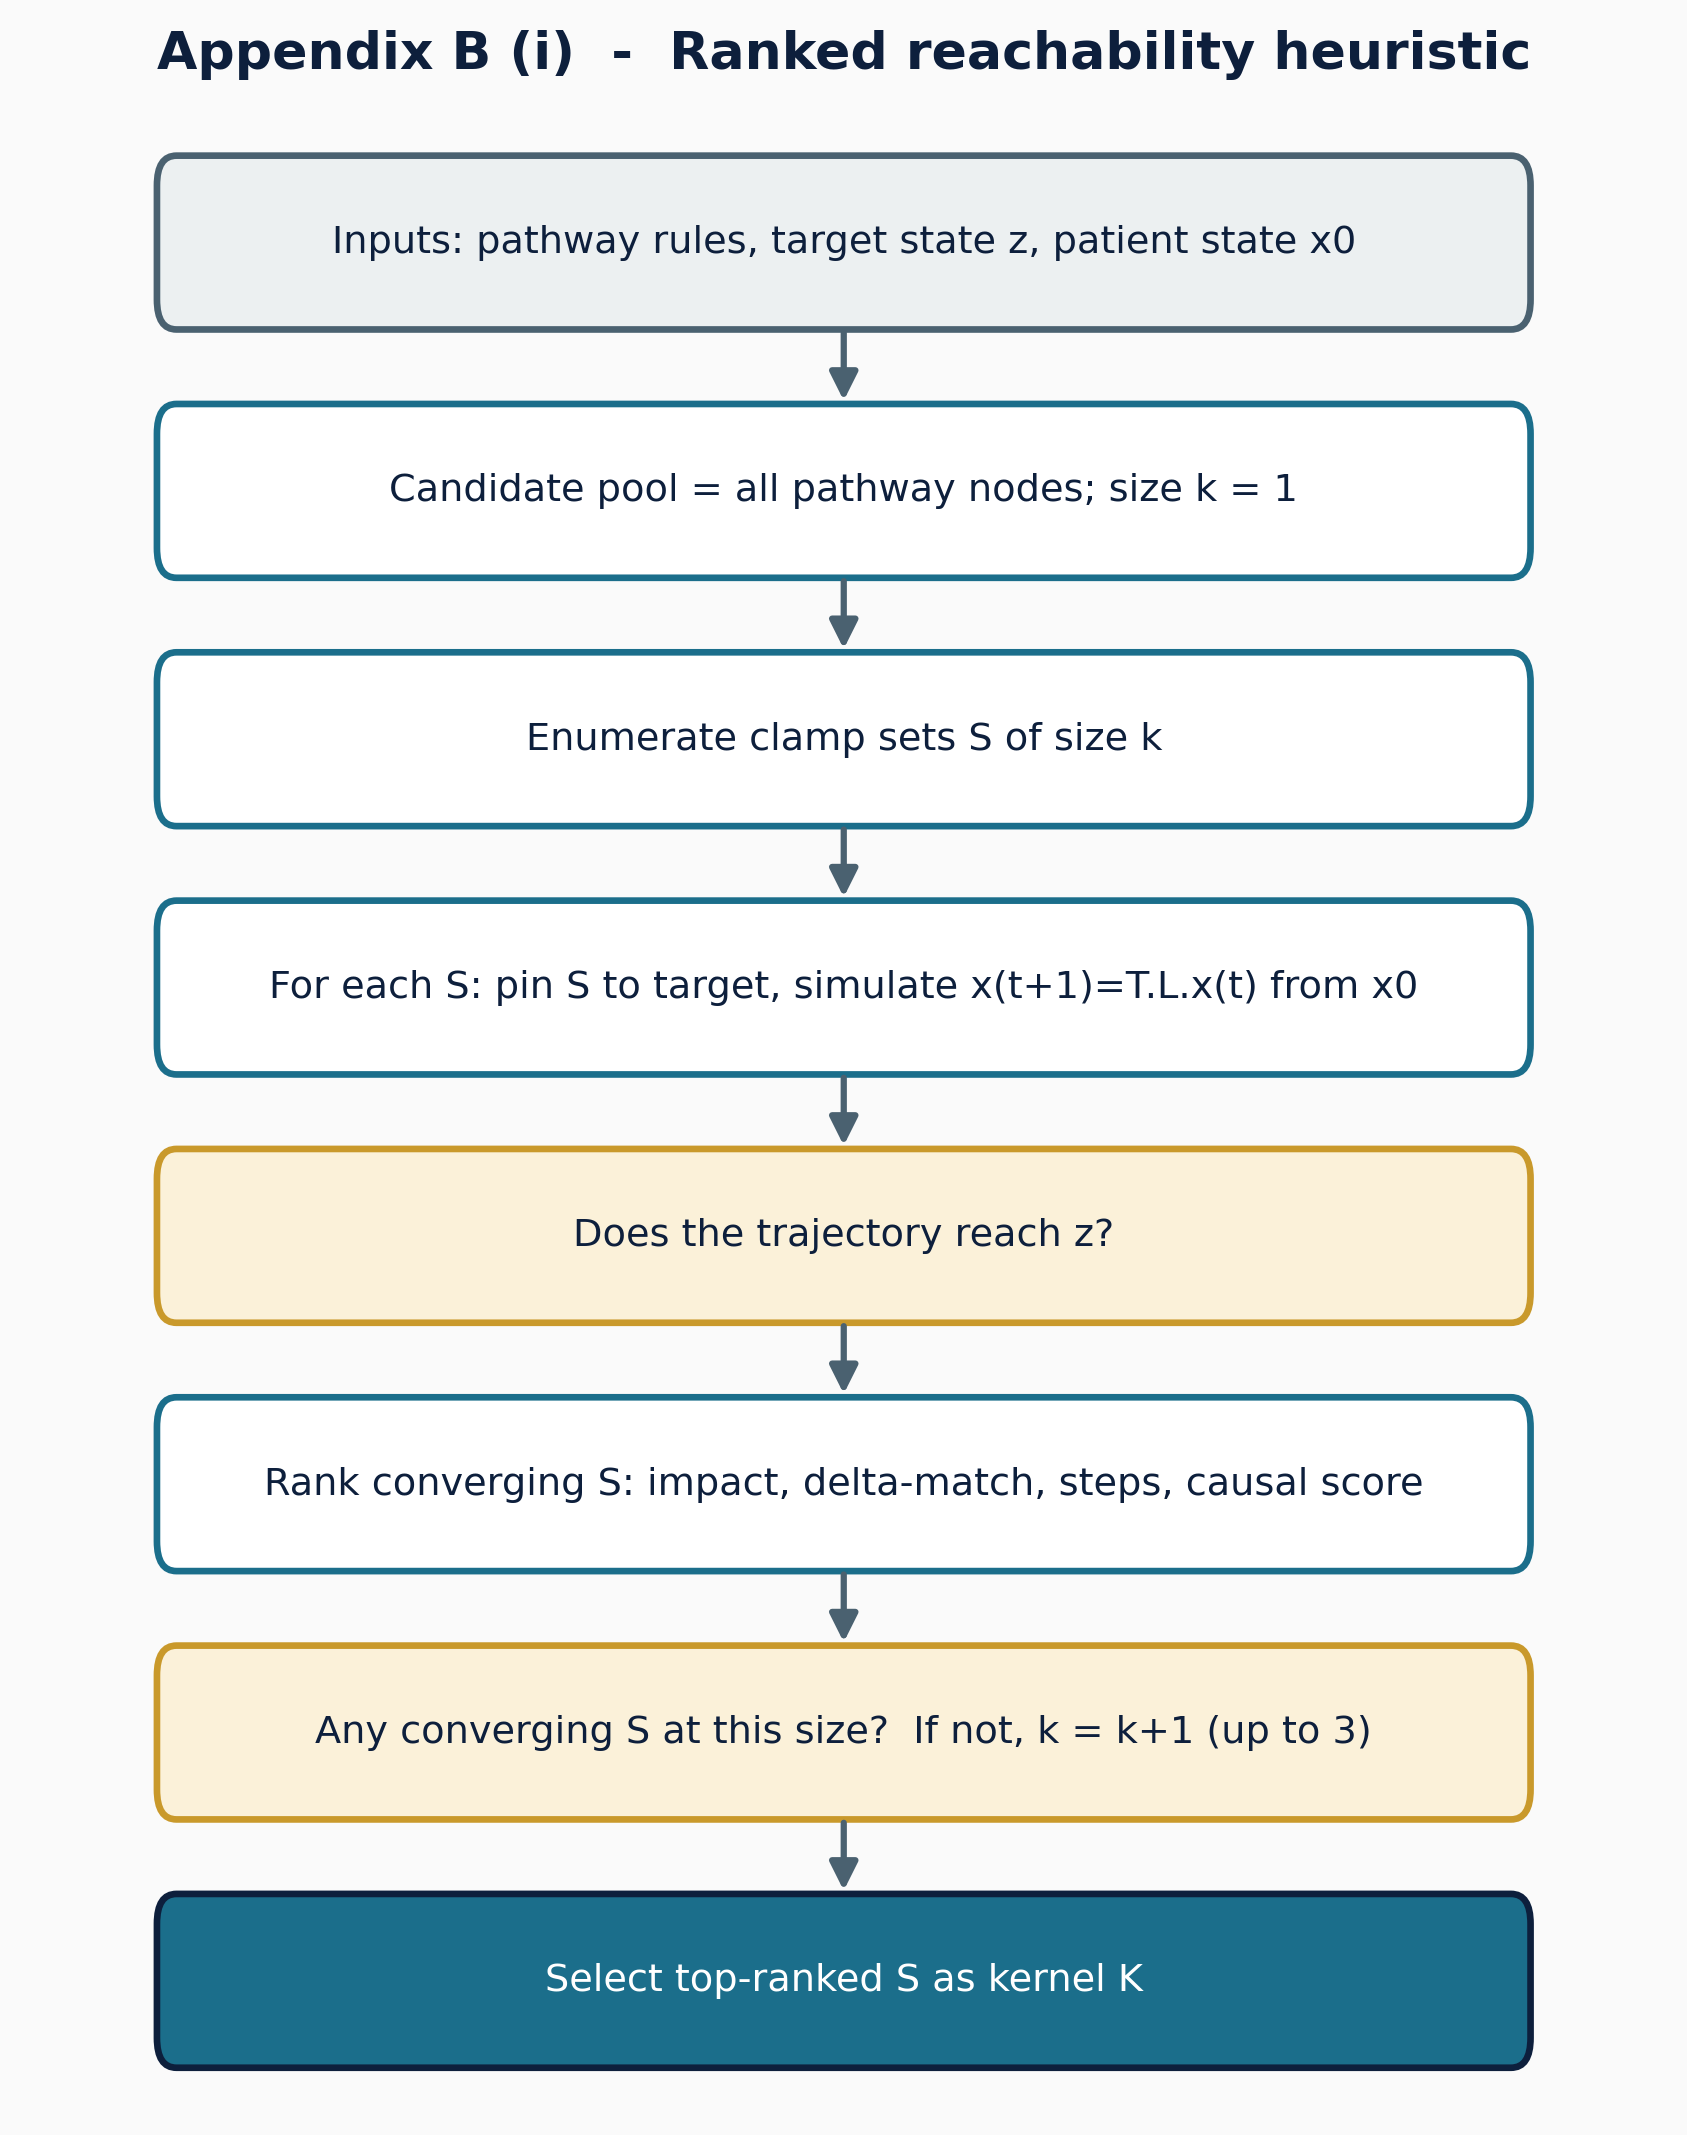
\includegraphics[width=0.6\textwidth]{figures/figC_flow_ranked.png}
\caption{\textbf{Ranked reachability heuristic (Tier~1).} Candidate clamp sets are enumerated by increasing size, each is simulated from the patient state, and converging sets are ranked by impact, then delta-match, then steps, then a causal score; the top set is the kernel. This is the heuristic that reproduces the earlier BBCN118 kernels.}
\label{fig:flowranked}
\end{figure}

\begin{figure}[H]
\centering
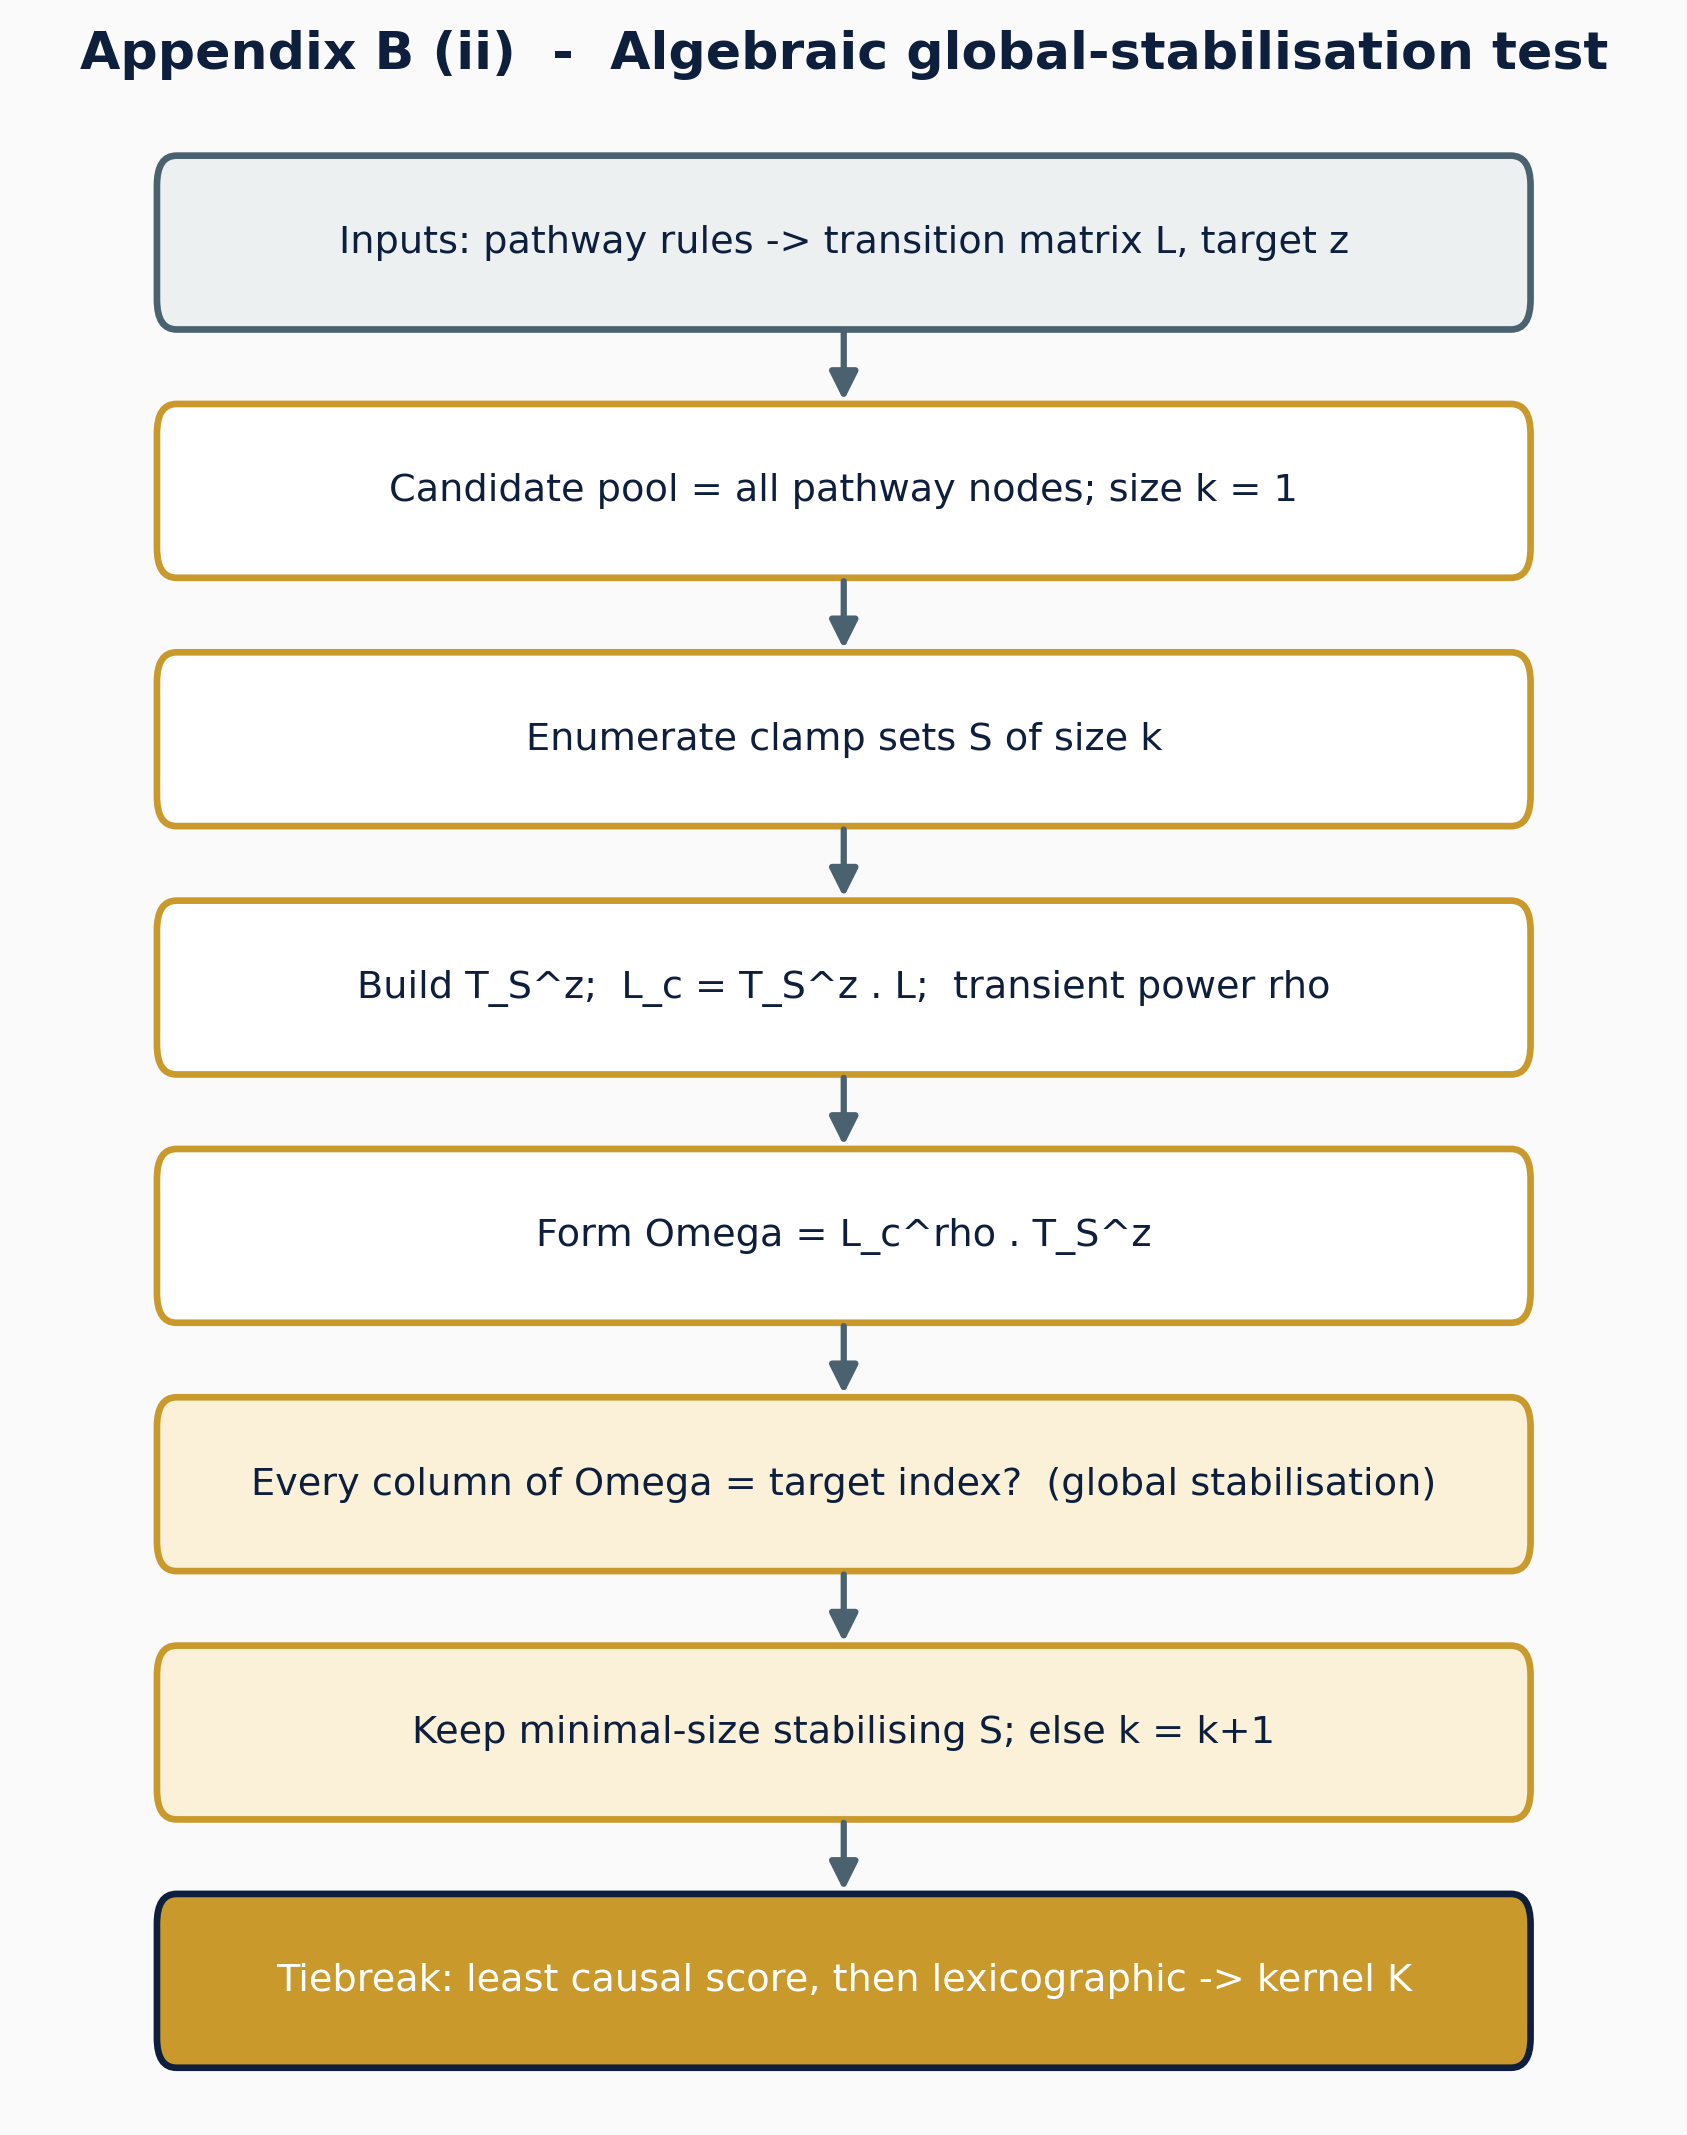
\includegraphics[width=0.6\textwidth]{figures/figC_flow_stabilize.png}
\caption{\textbf{Algebraic global-stabilisation test (Tier~1).} For each candidate clamp set $S$, the controlled operator $\Omega=L_c^{\rho}T_S^z$ is formed, and $S$ is accepted only if every column of $\Omega$ is the target index, that is, the clamp drives every pathway state to target, not only the patient's. Minimal-size accepted sets are kept and ties broken deterministically. This is the conservative, provable method used as the canonical kernel.}
\label{fig:flowstab}
\end{figure}

% Appendix C -- attributed restatement of the decomposition theorem of the prior preprint.
\section{The weak-coupling decomposition theorem (prior work)}
\label{app:theorem}

This appendix restates, for completeness, the pathway-decomposition theorem that the present
work positions itself against. The theorem and its proof are the contribution of the earlier
BBCN118 preprint~\cite{bhatti2026} (CC BY 4.0); the statement and proof sketch below are
reproduced and adapted from that work. They are included here so that the boundary identified
in Section~\ref{sec:32} can be read without consulting the source. The new content is the final
remark, which names the assumption the present network violates.

\paragraph{Setup.} Let a Boolean network with global update $x(t{+}1)=F(x(t))$ be partitioned into
$m$ pathway modules $P_1,\dots,P_m$, with module states $x_i$ and module targets $x_i^{*}$, so that
$x=(x_1,\dots,x_m)$ and $x^{*}=(x_1^{*},\dots,x_m^{*})$.

\paragraph{Theorem 1 (convergence under pathway decomposition).} Assume:
\begin{itemize}
\item[(A1)] \emph{Weak inter-pathway coupling:} $\displaystyle\max_{i\neq j}\left\|\partial F_i/\partial x_j\right\| < \varepsilon$, with $\varepsilon \ll 1$;
\item[(A2)] \emph{Local kernel effectiveness:} for each module $i$ there is a kernel $u_i$ that drives $x_i(t)\to x_i^{*}$ in finitely many steps; and
\item[(A3)] \emph{Modularity:} $F_i(x)\approx f_i\!\left(x_i, e_i(x)\right)$, where $e_i(x)$ collects the inputs $P_i$ receives from other modules.
\end{itemize}
Then the sequential application of the pathway kernels $u=\bigcup_{i=1}^{m} u_i$ drives the global
state into a neighbourhood of the target,
\[
x(t)\to \mathcal{N}_\delta(x^{*})=\{x : d_H(x,x^{*})\le \delta\},\qquad \delta = O(\varepsilon),
\]
where $d_H$ is the Hamming distance.

\paragraph{Proof sketch.} Take the weighted Hamming Lyapunov function
\[
V(x)=\sum_{i=1}^{m} w_i\, d_H\!\left(x_i,x_i^{*}\right),\qquad w_i>0 .
\]
$V$ is non-negative, integer-valued, bounded above by $\sum_i w_i|P_i|$, and zero exactly at $x^{*}$.
Intervening on module $k$ reduces its term by some $\alpha_k>0$ by (A2). By (A1) every other module
moves by at most $w_j\varepsilon|P_j|$, so
\[
\Delta V \le -\alpha_k + \varepsilon\sum_{j\neq k} w_j|P_j| ,
\]
which is strictly negative once $\varepsilon$ is small enough relative to $\alpha_k$. Because $V$ is
bounded below, strictly decreasing, and integer-valued, it reaches a minimum $V_{\min}$ in finitely
many steps, with $V_{\min}\le\delta=O(\varepsilon)$; at $\varepsilon=0$ the bound gives $V_{\min}=0$
and exact convergence. \hfill$\square$

\paragraph{Corollary 1 (convergence rate).} If each pathway kernel reduces the mismatch by at least
$\beta>0$ per intervention, the system reaches the neighbourhood in at most $T \le V(x(0))\,/\,(\beta/2)$
interventions.

\paragraph{Remark: why this paper is in the other regime.} The result holds only under assumption
(A1). The present BBCN network does not satisfy it. Its pathway-coupling graph carries a dominant
strongly-connected component of 16 of the 22 regulatory pathways (Section~\ref{sec:32}), so the
inter-module coupling is not small, the $O(\varepsilon)$ neighbourhood is not tight, and pathway-wise
stabilisation does not deliver joint reachability. That boundary is precisely what motivates modelling
the apoptosis core directly as the bistable switch of Setup~B. The full proof, including the explicit
$\varepsilon$ threshold, is given in the cited preprint and is not reproduced here.

% ------------------------------------------------------------
\begin{thebibliography}{99}
\bibitem{bhatti2026} Bhatti, A. I. From Pathway to Patient: Molecular Dysregulation as Basis for Minimal Sequential Intervention Strategy in Basal-Like Breast Cancer. \emph{Research Square} (2026). DOI: 10.21203/rs.3.rs-8942485/v1.
\bibitem{rafimanzelat2025} Rafimanzelat, M. R. Global stabilization of Boolean networks with applications to biomolecular network control. \emph{Sci. Rep.} \textbf{15}, 15201 (2025). DOI: 10.1038/s41598-025-97684-y.
\bibitem{zanudo2015} Za\~{n}udo, J. G. T. \& Albert, R. Cell fate reprogramming by control of intracellular network dynamics. \emph{PLoS Comput. Biol.} \textbf{11}(4), e1004193 (2015).
\bibitem{zanudo2013} Za\~{n}udo, J. G. T. \& Albert, R. An effective network reduction approach to find the dynamical repertoire of discrete dynamic networks. \emph{Chaos} \textbf{23}(2), 025111 (2013).
\bibitem{rozum2022} Rozum, J. C., Deritei, D., Park, K. H., Za\~{n}udo, J. G. T. \& Albert, R. pystablemotifs: Python library for attractor identification and control in Boolean networks. \emph{Bioinformatics} \textbf{38}, 1465--1466 (2022).
\bibitem{cheng2009} Cheng, D. \& Qi, H. Controllability and observability of Boolean control networks. \emph{Automatica} \textbf{45}, 1659--1667 (2009).
\bibitem{montagud2022} Montagud, A. et al. Patient-specific Boolean models of signalling networks guide personalised treatments. \emph{eLife} \textbf{11}, e72626 (2022).
\bibitem{beal2019} B\'{e}al, J., Montagud, A., Traynard, P., Barillot, E. \& Calzone, L. Personalization of logical models with multi-omics data allows clinical stratification of patients. \emph{Front. Physiol.} \textbf{9}, 1965 (2019).
\bibitem{wee2009} Wee, K. B. \& Aguda, B. D. Akt versus p53 in a network of oncogenes and tumour-suppressor genes regulating cell survival and death. \emph{PLoS ONE} \textbf{4}, e4407 (2009).
\bibitem{gao2005} Gao, T., Furnari, F. \& Newton, A. C. PHLPP: a phosphatase that directly dephosphorylates Akt. \emph{Mol. Cell} \textbf{18}, 13--24 (2005).
\bibitem{tarjan1972} Tarjan, R. Depth-first search and linear graph algorithms. \emph{SIAM J. Comput.} \textbf{1}, 146--160 (1972).
\bibitem{tcga2012} The Cancer Genome Atlas Network. Comprehensive molecular portraits of human breast tumours. \emph{Nature} \textbf{490}, 61--70 (2012).
\bibitem{metabric2012} Curtis, C. et al. The genomic and transcriptomic architecture of breast tumours (METABRIC). \emph{Nature} \textbf{486}, 346--352 (2012).
\bibitem{kauffman1969} Kauffman, S. A. Metabolic stability and epigenesis in randomly constructed genetic nets. \emph{J. Theor. Biol.} \textbf{22}, 437--467 (1969).
\bibitem{thomas1991} Thomas, R. Regulatory networks seen as asynchronous automata: a logical description. \emph{J. Theor. Biol.} \textbf{153}, 1--23 (1991).
\bibitem{albert2003} Albert, R. \& Othmer, H. G. The topology of the regulatory interactions predicts the expression pattern of the segment polarity genes in \emph{Drosophila melanogaster}. \emph{J. Theor. Biol.} \textbf{223}, 1--18 (2003).
\bibitem{saez2009} Saez-Rodriguez, J. et al. Discrete logic modelling as a means to link protein signalling networks with functional analysis of mammalian signal transduction. \emph{Mol. Syst. Biol.} \textbf{5}, 331 (2009).
\bibitem{morris2010} Morris, M. K., Saez-Rodriguez, J., Sorger, P. K. \& Lauffenburger, D. A. Logic-based models for the analysis of cell signaling networks. \emph{Biochemistry} \textbf{49}, 3216--3224 (2010).
\bibitem{helikar2012} Helikar, T. et al. The Cell Collective: toward an open and collaborative approach to systems biology. \emph{BMC Syst. Biol.} \textbf{6}, 96 (2012).
\bibitem{naldi2018} Naldi, A. et al. Logical modeling and analysis of cellular regulatory networks with GINsim 3.0. \emph{Front. Physiol.} \textbf{9}, 646 (2018).
\bibitem{fumia2013} Fumia, H. F. \& Martins, M. L. Boolean network model for cancer pathways: predicting carcinogenesis and targeted therapy outcomes. \emph{PLoS ONE} \textbf{8}, e69008 (2013).
\bibitem{vonderheyde2014} von der Heyde, S. et al. Boolean ErbB network reconstructions and perturbation simulations reveal individual drug response in different breast cancer cell lines. \emph{BMC Syst. Biol.} \textbf{8}, 75 (2014).
\bibitem{sgariglia2024} Sgariglia, D. et al. Optimizing therapeutic targets for breast cancer using Boolean network models. \emph{Comput. Biol. Chem.} \textbf{109}, 108022 (2024).
\bibitem{taoma2024} Taoma, K., Ruengjitchatchawalya, M., Liangruksa, M. \& Laomettachit, T. Boolean modeling of breast cancer signaling pathways uncovers mechanisms of drug synergy. \emph{PLoS ONE} \textbf{19}, e0298788 (2024).
\bibitem{zanudo2017} Gomez Tejeda Za\~{n}udo, J., Scaltriti, M. \& Albert, R. A network modeling approach to elucidate drug resistance mechanisms and predict combinatorial drug treatments in breast cancer. \emph{Cancer Converg.} \textbf{1}, 5 (2017).
\bibitem{fiedler2013} Fiedler, B., Mochizuki, A., Kurosawa, G. \& Saito, D. Dynamics and control at feedback vertex sets I: informative and determining nodes in regulatory networks. \emph{J. Dyn. Differ. Equ.} \textbf{25}, 563--604 (2013).
\bibitem{shmulevich2002} Shmulevich, I., Dougherty, E. R., Kim, S. \& Zhang, W. Probabilistic Boolean networks: a rule-based uncertainty model for gene regulatory networks. \emph{Bioinformatics} \textbf{18}, 261--274 (2002).
\end{thebibliography}

\end{document}
